% HISTORICAL TECHNICAL RECORD — NOT A CANONICAL CLAIM SOURCE.
% Current scope and claim boundaries are in PROJECT.md.
% =====================================================================
% Master Technical Report
% Image-Based Visual Servoing for High-Speed Multicopter Interception
% via Safe Reinforcement Learning
% =====================================================================
\documentclass[11pt]{article}

\usepackage[a4paper,margin=1in]{geometry}
\usepackage{graphicx}
\usepackage{amsmath,amssymb,bm}
\usepackage{booktabs}
\usepackage{multirow}
\usepackage{array}
\usepackage{xcolor}
\usepackage{hyperref}
\usepackage{caption}
\usepackage{subcaption}
\usepackage{float}
\usepackage{enumitem}
\usepackage{fancyhdr}
\usepackage{titlesec}

\hypersetup{colorlinks=true, linkcolor=blue!60!black,
            citecolor=green!50!black, urlcolor=blue!60!black}
\graphicspath{{./}}

\definecolor{boxgray}{RGB}{245,245,245}
\definecolor{accent}{RGB}{31,77,120}

\titleformat{\section}{\Large\bfseries\color{accent}}{\thesection}{1em}{}
\titleformat{\subsection}{\large\bfseries\color{accent!85!black}}{\thesubsection}{1em}{}

\pagestyle{fancy}\fancyhf{}
\lhead{\small IBVS Interception via Safe RL}
\rhead{\small Master Technical Report}
\cfoot{\thepage}

\newcommand{\stagebox}[1]{\vspace{2pt}\noindent\colorbox{boxgray}{%
\parbox{\dimexpr\linewidth-2\fboxsep}{\small #1}}\vspace{4pt}}

\title{\vspace{-1.2cm}\textbf{Image-Based Visual Servoing for High-Speed\\
Multicopter Interception via Safe Reinforcement Learning}\\[4pt]
\large A Staged Curriculum from Kinematic Validation to\\
Control-Barrier-Function Safety with In-Policy Projection}
\author{Project Master Technical Report}
\date{Compiled \today}

\begin{document}
\maketitle
\thispagestyle{fancy}

\begin{abstract}
\noindent
We present an end-to-end study of training a reinforcement-learning policy
for image-based visual servoing (IBVS) interception of a maneuvering aerial
target, progressing through a nine-step curriculum from a kinematic
pipeline-validation stage to a full six-degree-of-freedom (6-DOF)
multicopter with realistic perception, environmental wind, and
control-barrier-function (CBF) safety enforcement. The contribution is twofold.
First, a \emph{reproducible staged methodology}: each stage isolates a single
new source of difficulty (action semantics, observation realism, sensor
noise/delay, attitude dynamics, safety, disturbance), warm-started from the
previous stage, with deterministic 200-episode evaluation at a fixed seed.
Second, a \emph{rigorous safe-RL ablation}: we compare an external CBF-QP
safety filter against an in-policy differentiable CBF projection (``HardNet''),
and through a controlled multi-seed study (variance baseline $\rightarrow$
entropy/curriculum interventions $\rightarrow$ auxiliary feasibility loss
$\rightarrow$ $\lambda$ ablation) we show that the in-policy projection,
once its gradients are properly conditioned, attains the best worst-case
robustness ($36.7\%$ success under $\sim$92\% detection dropout and
$1.5\,$m/s wind) while preserving nominal performance ($\sim$91\%) and
hard attitude-safety guarantees ($\le 0.02\%$ limit-exceedance across
thousands of episodes). Every numeric result is taken from committed
evaluation logs.
\end{abstract}

\tableofcontents
\newpage

% =====================================================================
\section{Introduction and Problem Formulation}
% =====================================================================
\subsection{Motivation}
High-speed interception of an agile aerial target using only on-board vision
is a canonical safety-critical control problem: the interceptor must keep the
target inside its camera field of view (FOV) while closing distance rapidly,
all under partial observability, sensor noise, and actuator limits. We adopt
the image-based visual-servoing (IBVS) formulation of Yang et al.
(arXiv:2404.08296), in which feedback is defined directly on the image plane,
and we learn the guidance policy with Proximal Policy Optimization (PPO).

\subsection{Coordinate Conventions and Notation}
We use the North-East-Down (NED) earth-fixed coordinate system (EFCS), with
$z$ pointing down. The camera frame has $x$ right, $y$ down, $z$ forward
(optical axis). Key symbols:
\begin{itemize}[nosep]
  \item $\bar{\mathbf{p}}=(\bar p_x,\bar p_y)$ --- normalized image
  coordinates of the target.
  \item $\mathbf{L}_s\in\mathbb{R}^{2\times6}$ --- IBVS interaction matrix
  (image Jacobian) relating camera spatial velocity to image-feature velocity.
  \item $\mathbf{u}=(a_x,a_y,a_z,\dot\psi)$ --- 4-D action: body-frame
  acceleration commands and yaw rate, normalized to $[-1,1]$.
  \item $h_i(\mathbf{x})$ --- CBF barrier functions (FOV-horizontal,
  FOV-vertical, pitch, roll).
\end{itemize}

\subsection{The Staged Curriculum}
Table~\ref{tab:roadmap} summarizes the curriculum. Each row introduces
exactly one new difficulty, enabling clean attribution of performance changes.
Figure~\ref{fig:progression} plots the headline success rate across stages.

\begin{table}[H]\centering\small
\caption{Staged curriculum. ``Warm'' = warm-started from the previous stage.}
\label{tab:roadmap}
\begin{tabular}{@{}llll@{}}
\toprule
Stage & New difficulty & Train from & Headline success \\
\midrule
1a & Pipeline validation (kinematic, full obs) & fresh & 100\% \\
1b & Acceleration control + action smoothing & warm & $>$90\% \\
2a & Vision-only observation & fresh & $\sim$70\% \\
2b & Noise + delay + DKF observer & warm & 62\% \\
3a & First-order dynamics + attitude coupling & fresh & 66\% (mild) \\
3b & Full 6-DOF + SO(3) PD attitude control & warm & \textbf{96.5\%} (mild) \\
4a & CBF safety (filter \emph{and} in-policy) & fine-tune & 89--92\% \\
4b & Realistic perception + wind (DR) & warm & 91\% nominal \\
\bottomrule
\end{tabular}
\end{table}

\begin{figure}[H]\centering
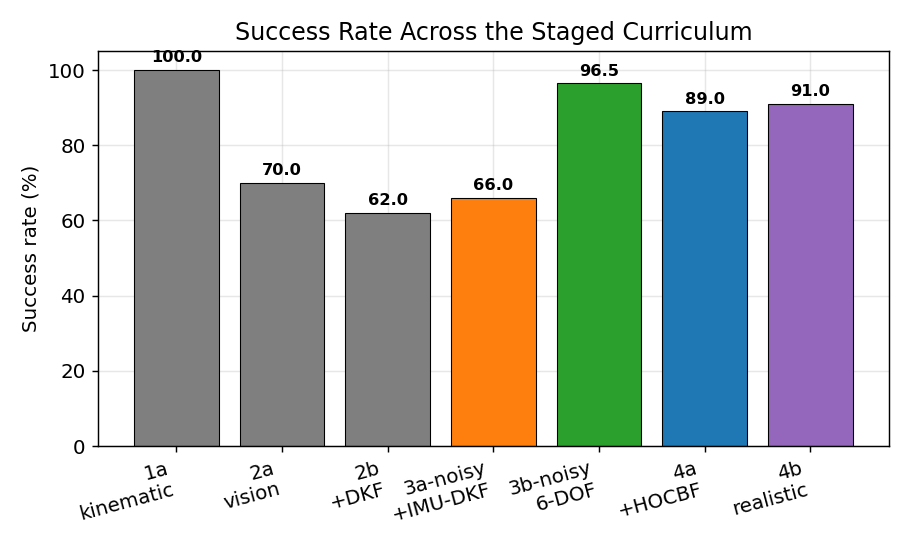
\includegraphics[width=0.82\linewidth]{figures/progression.png}
\caption{Success rate along the staged curriculum. Grey = early kinematic
stages; orange = noisy kinematic; green = 6-DOF; blue = safety; purple =
realistic perception. The 3a$\rightarrow$3b jump is the dynamics-fidelity
effect (\S\ref{sec:3b}).}
\label{fig:progression}
\end{figure}

\subsection{Common Experimental Infrastructure}
\stagebox{\textbf{Algorithm:} PPO (Stable-Baselines3), MLP policy.
\textbf{Vectorization:} 16 parallel environments. \textbf{Rollout:}
$n_\text{steps}=2048$, batch 64, 10 epochs, $\gamma=0.99$,
$\lambda_\text{GAE}=0.95$, clip $0.2$. \textbf{Timestep:} $dt=20\,$ms (50 Hz).
\textbf{Evaluation:} deterministic policy, 200 episodes at fixed eval
seed~1000 unless noted. \textbf{Late-stage:} linear learning-rate decay
$3\times10^{-4}\rightarrow0$ to mitigate the overtraining pattern observed
throughout (best checkpoint typically precedes the final one).}

% =====================================================================
\section{Mathematical Formulations}
\label{sec:math}
% =====================================================================
This section gives the complete, implementation-faithful mathematical
specification of every model, filter, controller, and safety operator used
in the project. The stage chapters (\S6--\S12) reference these formulations
and report experimental validation. All equations below correspond directly
to the committed source (\texttt{models/}, \texttt{observers/}, \texttt{safety/}).

\subsection{System State and the Pinhole Measurement Model}
\label{sec:state}
Let the earth-fixed (NED) position of interceptor and target be
$\mathbf p,\,\mathbf p_t\in\mathbb R^3$ with $z$ down. The relative position
is $\mathbf p_r=\mathbf p-\mathbf p_t$ and the range $d=\lVert\mathbf p_r\rVert$.
Let $R_b^e\in SO(3)$ be the body-to-earth rotation and $R_c^b$ the fixed
body-to-camera rotation (a $-\pi/2$ pitch placing the optical axis along body
$+x$). A target point in the camera frame is
\begin{equation}
\mathbf p^c = R_c^b\,(R_b^e)^\top\,(\mathbf p_t-\mathbf p)
= [x_c,\,y_c,\,z_c]^\top .
\end{equation}
The normalized pinhole projection and field-of-view (FOV) test are
\begin{equation}
\bar{\mathbf p}=\Big[\tfrac{x_c}{z_c},\,\tfrac{y_c}{z_c}\Big]^\top,
\qquad
\text{in-FOV}\;\Leftrightarrow\;
\Big|\arctan\tfrac{x_c}{z_c}\Big|\le\tfrac{\alpha_h}{2}\;\wedge\;
\Big|\arctan\tfrac{y_c}{z_c}\Big|\le\tfrac{\alpha_v}{2},
\label{eq:fov}
\end{equation}
with horizontal/vertical FOV $\alpha_h=70^\circ$, $\alpha_v=55^\circ$. The
FOV margin $m_\text{FOV}=\min(1-\tfrac{|\arctan(x_c/z_c)|}{\alpha_h/2},\,
1-\tfrac{|\arctan(y_c/z_c)|}{\alpha_v/2})\in[0,1]$ ($1$ = centered, $0$ = edge).

\subsection{Interaction Matrix (Image Jacobian)}
For a point feature at $\bar{\mathbf p}=(\bar p_x,\bar p_y)$ and depth $z_c$,
the IBVS interaction matrix $\mathbf L_s\in\mathbb R^{2\times6}$ maps the
camera spatial velocity $[\mathbf v_c;\bm\omega_c]$ to image-feature velocity
$\dot{\bar{\mathbf p}}=\mathbf L_s[\mathbf v_c;\bm\omega_c]$:
\begin{equation}
\mathbf L_s=\begin{bmatrix}
-\tfrac{1}{z_c} & 0 & \tfrac{\bar p_x}{z_c} & \bar p_x\bar p_y & -(1+\bar p_x^2) & \bar p_y\\[2pt]
0 & -\tfrac{1}{z_c} & \tfrac{\bar p_y}{z_c} & 1+\bar p_y^2 & -\bar p_x\bar p_y & -\bar p_x
\end{bmatrix}.
\label{eq:Ls}
\end{equation}
The rotational sub-block (columns 4--6) is depth-independent; this property
underlies both the depth estimator (\S\ref{sec:depth}) and the IMU-aware DKF
prediction (\S\ref{sec:dkf}).

\subsection{Target Dynamics}
\label{sec:target}
The target is a point mass integrated at $dt$ with one of four maneuver modes,
$\dot{\mathbf p}_t=\mathbf v_t,\;\dot{\mathbf v}_t=\mathbf a_t$:
\begin{itemize}[nosep]
\item \textbf{Constant velocity:} $\mathbf a_t=\mathbf 0$.
\item \textbf{Sinusoidal evasion:} lateral acceleration
$\mathbf a_t=A\,\omega^2\sin(\omega t+\phi)\,\hat{\mathbf e}_\perp$ on an axis
$\hat{\mathbf e}_\perp$ perpendicular to the initial velocity, amplitude
$A=3\,$m, frequency $\omega=1.5\,$rad/s.
\item \textbf{Circular:} orbit of radius $R=15\,$m at rate $\omega=0.5\,$rad/s,
$\mathbf a_t=-\omega^2(\mathbf p_t-\mathbf c)$.
\item \textbf{Random aggressive:} $\mathbf a_t$ resampled uniformly in
$\lVert\mathbf a_t\rVert\le a_t^{\max}$ every $25$ steps.
\end{itemize}
The target is observed only through its projection \eqref{eq:fov}; no target
state enters the policy observation directly (it appears only via $\bar{\mathbf p}$
and, during \emph{training}, via the privileged range $d$ in the reward).

\subsection{Interceptor Dynamics --- Two Models}
\label{sec:dyn}
\paragraph{(A) Kinematic first-order model (Stages 1--3a).}
The action $\mathbf u=(a_x,a_y,a_z,\dot\psi)$ is a body-frame acceleration
command plus yaw rate. Body velocity follows a first-order lag toward the
commanded velocity $\mathbf v^\star=\mathrm{clip}(\mathbf v_b+\mathbf a\,dt,
v_{\max})$:
\begin{align}
\mathbf v_b &\leftarrow \mathbf v_b+\alpha_v(\mathbf v^\star-\mathbf v_b),
&\alpha_v&=\min(dt/\tau_v,1),\;\tau_v=0.15\,\text{s},\\
\theta_\text{des}&=-\arctan\!\tfrac{a_x}{g},\quad
\phi_\text{des}=\arctan\!\tfrac{a_y}{g}, &
\theta&\leftarrow\theta+\alpha_\theta(\theta_\text{des}-\theta),\;
\tau_\theta=0.3\,\tau_v,\\
\dot\psi&\leftarrow\dot\psi+\alpha_\psi(\dot\psi_\text{cmd}-\dot\psi),&
\psi&\leftarrow\psi+\dot\psi\,dt,\;\tau_\psi=0.10\,\text{s},
\end{align}
with attitude limits $|\theta|,|\phi|\le35^\circ$. The EFCS velocity is
$\mathbf v=R_b^e\mathbf v_b$ and $\mathbf p\leftarrow\mathbf p+\mathbf v\,dt$.
The defining feature is the acceleration--attitude coupling
$\theta_\text{des}=-\arctan(a_x/g)$: aggressive forward acceleration pitches
the nose down, tilting the camera and threatening FOV loss.

\paragraph{(B) Full 6-DOF Newton--Euler model (Stages 3b--4b).}
\label{sec:6dof}
The state is $(\mathbf p,\mathbf v,R_b^e,\bm\omega_b,f)$ with EFCS position
/velocity, attitude, body angular rate, and scalar thrust. With mass $m$,
gravity $\mathbf g=[0,0,g]^\top$, and thrust acting along body $-z$:
\begin{align}
\dot{\mathbf p}&=\mathbf v, &
\dot{\mathbf v}&=\mathbf g-\tfrac{f}{m}R_b^e\mathbf e_3, \label{eq:newton}\\
\dot R_b^e&=R_b^e\,[\bm\omega_b]_\times, &
[\bm\omega_b]_\times&=\text{skew}(\bm\omega_b),
\end{align}
integrated by composing $R_b^e$ with the incremental rotation
$\exp([\bm\omega_b\,dt]_\times)$ (via a quaternion, avoiding Euler
singularities). The motor and rate loops are first-order:
\begin{equation}
f\leftarrow f+\tfrac{dt}{\tau_m}(f_d-f),\qquad
\bm\omega_b\leftarrow\bm\omega_b+\tfrac{dt}{\tau_r}(\bm\omega_d-\bm\omega_b),
\quad \tau_m=\tau_r=50\,\text{ms},
\end{equation}
with $\bm\omega_b$ saturated to $\omega_{\max}=4\,$rad/s and
$f\in[0,f_{\max}]$, $f_{\max}=3mg$ (thrust-to-weight 3). The desired thrust
$f_d$ and body rate $\bm\omega_d$ come from the SO(3) attitude controller
(\S\ref{sec:so3}). Parameters: $m=1\,$kg, $J=\mathrm{diag}(0.01,0.01,0.02)\,$kg\,m$^2$.

\subsection{Depth Estimator (Inverse-Depth Kalman Filter)}
\label{sec:depth}
Depth is estimated in inverse-depth coordinates $\rho=1/z_c$, which linearizes
the translational image-velocity relation. Subtracting the (depth-independent)
rotational contribution from the measured image velocity gives the
translational residual $\dot{\bar{\mathbf p}}_\text{tr}=
\dot{\bar{\mathbf p}}-\mathbf L_\text{rot}\bm\omega_c$, and with
$\mathbf b=\mathbf B(\bar{\mathbf p})\,\mathbf v_\text{rel}^c$ (where
$\mathbf B=[\,\mathbf I_2\;\;-\bar{\mathbf p}\,]$) the relation
$\dot{\bar{\mathbf p}}_\text{tr}=\rho\,\mathbf b$ is \emph{linear} in $\rho$.
A scalar Kalman filter then runs
\begin{equation}
\rho^-=\rho,\;\;P^-=P+Q;\quad
K=\tfrac{P^- \mathbf b^\top}{\mathbf b P^-\mathbf b^\top+R},\;\;
\rho\leftarrow\rho^-+K(\dot{\bar{\mathbf p}}_\text{tr}-\rho^-\mathbf b),\;\;
P\leftarrow(1-K\mathbf b)P^-,
\end{equation}
with $\rho$ clamped to $[\rho_{\min},\rho_{\max}]=[0.005,2]$ (i.e.
$z_c\in[0.5,200]\,$m) and the update gated by an observability threshold
$\lVert\mathbf b\rVert^2>\epsilon$.

\subsection{Disturbance Kalman Filter (Image-Plane State, Delay-Compensated)}
\label{sec:dkf}
The DKF estimates the current image-plane state
$\mathbf x=[\bar p_x,\bar p_y,\dot{\bar p}_x,\dot{\bar p}_y]^\top$ from noisy,
$D$-step-delayed measurements. Constant-velocity process and position-only
measurement models:
\begin{equation}
\mathbf x_{k+1}=F\mathbf x_k+\mathbf w_k,\quad
F=\begin{bmatrix}\mathbf I_2 & dt\,\mathbf I_2\\ \mathbf 0 & \mathbf I_2\end{bmatrix},
\qquad
\mathbf z_k=H\mathbf x_{k-D}+\mathbf n_k,\quad H=[\mathbf I_2\;\;\mathbf 0],
\end{equation}
$\mathbf w_k\sim\mathcal N(0,Q)$, $\mathbf n_k\sim\mathcal N(0,R)$,
$Q=\mathrm{diag}(\sigma_p^2,\sigma_p^2,\sigma_v^2,\sigma_v^2)$ with a
deliberately large velocity process noise $\sigma_v=0.5$ (disturbance-aware
tracking of maneuvers without an explicit target model).
\paragraph{Prediction (standard):}
$\mathbf x\leftarrow F\mathbf x$, $P\leftarrow FPF^\top+Q$.
\paragraph{Prediction (IMU-aware upgrade).} The camera ego-motion induces an
image velocity $\dot{\bar{\mathbf p}}_\text{cam}=\mathbf L_s
[\mathbf v_c;\bm\omega_c]$ that changes \emph{abruptly} during aggressive
attitude changes --- precisely when the constant-velocity assumption fails.
We therefore feed forward only the \emph{change} in the camera contribution,
applying CV to the (slowly-varying) target residual:
\begin{equation}
\Delta_\text{cam}=\dot{\bar{\mathbf p}}_{\text{cam},k}-\dot{\bar{\mathbf p}}_{\text{cam},k-1},\quad
\dot{\bar{\mathbf p}}\!\mathrel{+}=\!\Delta_\text{cam},\quad
\bar{\mathbf p}\!\mathrel{+}=\!\tfrac12 dt\,\Delta_\text{cam}.
\end{equation}
\paragraph{Delay-compensated update.} The measurement $\mathbf z_k$ pertains to
time $k\!-\!D$. Using the buffered prediction $\mathbf x_{k-D}$ and covariance
$P_{k-D}$ for the innovation, the gain is applied to the \emph{current} state
(a small-$D$ approximation):
\begin{equation}
\mathbf y=\mathbf z_k-H\mathbf x_{k-D},\;\;
S=HP_{k-D}H^\top+R,\;\;
K=P\,H^\top S^{-1},\;\;
\mathbf x\leftarrow\mathbf x+K\mathbf y,
\end{equation}
with the Joseph-form covariance update
$P\leftarrow(\mathbf I-KH)P(\mathbf I-KH)^\top+KRK^\top$ for numerical
stability. The 4-D DKF is the project's \emph{perception ceiling}: it saturates
between mild ($D{=}1,\sigma{=}.015$) and full ($D{=}3,\sigma{=}.03$) noise
regardless of dynamics fidelity (\S\ref{sec:3a},\ref{sec:3b}).

% =====================================================================
\section{Control and Safety Framework}
\label{sec:control}
% =====================================================================
\subsection{SO(3) Geometric Attitude Controller}
\label{sec:so3}
For the 6-DOF model, the policy's body-acceleration command $\mathbf a_b$ is
realized by a geometric controller on $SO(3)$ (Lee et al.\ 2010). Lift the
command to EFCS, $\mathbf a_d=R_b^e\mathbf a_b$, and form the required thrust
force $\mathbf f_\text{req}=m(\mathbf a_d-\mathbf g)$. Its magnitude and
direction set the desired thrust and tilt:
\begin{equation}
f_d=\mathrm{clip}(\lVert\mathbf f_\text{req}\rVert,0,f_{\max}),\qquad
\hat{\mathbf n}_{f_d}=\mathbf f_\text{req}/\lVert\mathbf f_\text{req}\rVert .
\end{equation}
The desired rotation $R_d=R_\text{tilt}R_b^e$ is the minimal tilt aligning the
current thrust axis $-R_b^e\mathbf e_3$ with $\hat{\mathbf n}_{f_d}$
(Rodrigues' formula on the axis $\hat{\mathbf n}_\text{cur}\times\hat{\mathbf n}_{f_d}$).
The attitude error and PD body-rate command are
\begin{equation}
\mathbf e_R=\tfrac12\big(R_d^\top R_b^e-(R_b^e)^\top R_d\big)^\vee,\qquad
\bm\omega_d=-k_\text{att}\,\mathbf e_R,\quad k_\text{att}=6,
\label{eq:so3}
\end{equation}
where $(\cdot)^\vee$ is the inverse hat (skew$\rightarrow$vector) map. The yaw
component is overridden by the policy's direct yaw-rate command,
$\omega_{d,z}=\dot\psi_\text{cmd}$, and $\bm\omega_d$ is saturated to
$\omega_{\max}$. The pair $(f_d,\bm\omega_d)$ then drives the first-order motor
and rate loops of \S\ref{sec:6dof}. This geometric controller produces
markedly smoother attitude responses than the kinematic $\arctan(a/g)$
coupling, which is the mechanism behind the large 3a$\rightarrow$3b gain.

\subsection{Control Barrier Functions and the Safe Polytope}
\label{sec:cbf}
We enforce four safety constraints as zeroing CBFs $h_i(\mathbf x)\ge0$ with
the smooth squared form (nonzero gradient at the boundary, the regularity
condition for forward invariance):
\begin{align}
h_\text{hfov}&=\tan^2\!\tfrac{\alpha_h}{2}-\bar p_x^2, &
h_\text{vfov}&=\tan^2\!\tfrac{\alpha_v}{2}-\bar p_y^2,\\
h_\text{pitch}&=\theta_{\max,\text{eff}}^2-\theta^2, &
h_\text{roll}&=\phi_{\max,\text{eff}}^2-\phi^2,
\end{align}
where $\theta_{\max,\text{eff}}=\theta_{\max}-\delta_s$ uses an inner safety
margin $\delta_s$ (default $0.10\,$rad) absorbing the proxy--truth mismatch
below. The safe set is the intersection
$\mathcal C(\mathbf x)=\{\,\mathbf u: A(\mathbf x)\mathbf u\ge \mathbf b(\mathbf x),\,
\mathbf u\in[-1,1]^4\,\}$, a polytope. The continuous-time CBF condition
$L_f h_i+L_g h_i\,\mathbf u+\alpha_i h_i\ge0$ rearranges to the affine row
$A_i\mathbf u\ge b_i$ with $A_i=L_g h_i$ and $b_i=-L_f h_i-\alpha_i h_i$.

\paragraph{Relative degree and the proxy linearization.} In the true 6-DOF
system the action (acceleration / yaw-rate) reaches the FOV and attitude
outputs only through the attitude-tracking lag and Newton integration --- a
relative degree $\ge2$, for which $L_g h_i\equiv0$ and the plain CBF-QP is
ill-posed. We adopt a \emph{control-affine proxy}: pitch and roll track
$\theta_\text{des}=-a_x/g$, $\phi_\text{des}=a_y/g$ through a single
$\tau_r$ lag, rendering all four constraints relative-degree-1 with
closed-form Lie derivatives. For the attitude barriers,
$\dot\theta=\tfrac1{\tau_r}(-a_x/g-\theta)$ gives
\begin{equation}
L_f h_\text{pitch}=\tfrac{2\theta^2}{\tau_r},\qquad
L_g h_\text{pitch}=\Big[\tfrac{2\theta}{g\tau_r},0,0,0\Big],
\end{equation}
and symmetrically for roll ($a_y$, with sign flip). For the FOV barriers the
$\mathbf u$-dependence flows through $\bm\omega_c=R_c^b\bm\omega_b$ with
$\bm\omega_b$ a function of $(a_x,a_y,\dot\psi)$; writing the per-step image
velocity $\dot{\bar{\mathbf p}}=\mathbf L_s[\mathbf v_\text{rel}^c;\bm\omega_c]$
and differentiating $h_\text{hfov}=\tan^2(\cdot)-\bar p_x^2$,
\begin{equation}
L_f h_\text{hfov}=-2\bar p_x\,\dot{\bar p}_{x,\text{drift}},\qquad
L_g h_\text{hfov}=-2\bar p_x\,\big[\mathbf L_\text{rot}R_c^b M\big]_{0,:},
\end{equation}
where $M$ is the constant Jacobian $\partial\bm\omega_b/\partial\mathbf u$ of
the proxy. FOV rows are deactivated ($A_i{=}0$) when the target is out of
frame. Because the proxy is first-order while the truth is second-order, the
proxy responds \emph{faster} than reality; the inner margin $\delta_s$ and a
large class-$\mathcal K$ rate $\alpha$ absorb the mismatch, and the empirical
attitude-limit exceedance stays $\le0.02\%$ of steps across thousands of
episodes.

\paragraph{The CBF-QP (external filter, Stage 4a.3).} Given the RL action
$\mathbf u_\text{RL}$, the minimally-invasive safe action solves
\begin{equation}
\mathbf u_\text{safe}=\arg\min_{\mathbf u}\tfrac12\lVert\mathbf u-\mathbf u_\text{RL}\rVert^2
\;\;\text{s.t.}\;\; A\mathbf u\ge\mathbf b,\;\mathbf u\in[-1,1]^4,
\label{eq:cbfqp}
\end{equation}
a 4-variable, $\le12$-constraint QP solved with \texttt{quadprog} in
$\sim0.15\,$ms. With a bisection fallback if \eqref{eq:cbfqp} is infeasible
(deep corners of the action box).

\subsection{HardNet: Differentiable In-Policy Projection}
\label{sec:hardnetmath}
HardNet replaces the external filter by embedding the projection onto
$\mathcal C(\mathbf x)$ \emph{inside} the policy, so gradients propagate
through it during PPO. The network emits $\mathbf u_\text{raw}$ and the policy
mean is the Euclidean projection
\begin{equation}
\mathbf u_\text{safe}=\Pi_{\mathcal C(\mathbf x)}(\mathbf u_\text{raw})
=\arg\min_{\mathbf u\in\mathcal C(\mathbf x)}\tfrac12\lVert\mathbf u-\mathbf u_\text{raw}\rVert^2 .
\end{equation}
Since $\mathcal C$ is an intersection of half-spaces and the box, we compute
$\Pi$ by \textbf{Dykstra's alternating projection}, which (unlike plain POCS)
converges to the true Euclidean projection. With correction terms
$\mathbf p^{(i)},\mathbf q$ initialized to zero, each sweep projects onto every
active half-space $\{\mathbf u:A_i\mathbf u\ge b_i\}$,
\begin{equation}
\mathbf y=\mathbf u+\mathbf p^{(i)},\quad
\mathbf u'=\mathbf y+\frac{\max(0,\,b_i-A_i\mathbf y)}{\lVert A_i\rVert^2}A_i^\top,\quad
\mathbf p^{(i)}\leftarrow\mathbf y-\mathbf u',\quad\mathbf u\leftarrow\mathbf u',
\end{equation}
followed by a box projection $\mathbf u\leftarrow\mathrm{clip}(\mathbf u+\mathbf q,-1,1)$,
$\mathbf q\leftarrow(\mathbf u+\mathbf q)-\mathbf u$, for $K{=}20$ sweeps. Each
elementary projection is piecewise-linear and differentiable, so
$\partial\mathbf u_\text{safe}/\partial\mathbf u_\text{raw}$ is the product of
the active-face projectors: it equals $\mathbf I$ on the interior (gradient
passes cleanly) and drops rank along active constraint normals (the gradient
pathology motivating Intervention~D, \S\ref{sec:hardnet}). The per-step
coefficients $(A,\mathbf b)$ are appended to the observation
($16\!\rightarrow\!36$-D) by a context wrapper; a slicing feature-extractor
keeps the network conditioned on only the 16-D base observation so weights
remain interchangeable with the unconstrained MLP policy (enabling warm-start).
Crucially, the executed and reward-relevant action is always
$\mathbf u_\text{safe}$, so the projection can neither produce unsafe behavior
nor (by itself) degrade task performance --- it reshapes only the internal
pre-image.

\paragraph{Intervention D --- auxiliary feasibility loss.} To keep the
projection Jacobian full-rank (healthy gradients) the PPO objective is
augmented with
\begin{equation}
\mathcal L=\mathcal L_\text{PPO}
+\lambda\,\mathbb E\big[\lVert\mathbf u_\text{raw}-\mathbf u_\text{safe}\rVert^2\big],
\end{equation}
which pulls $\mathbf u_\text{raw}$ toward feasibility so the projection
approaches the identity. The weight $\lambda$ trades a ``lazy policy''
(over-conservative at large $\lambda$) against gradient health; the ablation
(\S\ref{sec:hardnet}) locates the Pareto frontier.

\subsection{Reward Function (Canonical Form)}
\label{sec:reward}
All stages share the reward template below; stage-specific weights and gating
are noted in each chapter. With $\bar{\mathbf p}$ the image error, $d$ the
\emph{privileged} range (training-only ``teacher'' signal, never in the
observation), and $\mathbf a$ the normalized action:
\begin{align}
r &= \underbrace{w_\text{img}\,e^{-k_1\lVert\bar{\mathbf p}\rVert^2}\max\!\big(0,1-\tfrac{d}{d_\text{cut}}\big)\mathbb 1_\text{FOV}}_{\text{distance-gated centering}}
\;+\;\underbrace{w_\text{app}(d_{k-1}-d_k)}_{\text{approach}}
\;+\;\underbrace{w_\text{dist}\tfrac{d}{d_\text{norm}}}_{\text{anti-loiter}}\notag\\
&\quad+\,\underbrace{w_\text{brake}\lVert\mathbf v_b\rVert\tfrac{(d_b-d)^+}{d_b}}_{\text{terminal braking}}
\;+\;\underbrace{w_\text{fov}\,\mathbb 1_{\neg\text{FOV}}}_{\text{FOV loss}}
\;+\;\underbrace{w_\text{bnd}(1-m_\text{FOV})^2\mathbb 1_\text{FOV}}_{\text{boundary}}\notag\\
&\quad+\,w_\text{eff}\lVert\mathbf a\rVert^2
+ w_\text{jerk}\lVert\mathbf a-\mathbf a_{k-1}\rVert^2
+ w_\text{att}\big(\tilde\theta^2+\tilde\phi^2\big)
+ w_\text{time}
+ w_\text{int}\mathbb 1_\text{success},
\label{eq:reward}
\end{align}
with $\tilde\theta=\theta/\theta_{\max}$, $\tilde\phi=\phi/\phi_{\max}$,
success when $d<d_\text{succ}=2\,$m, and FOV-loss termination after
$15$ consecutive out-of-frame steps. The canonical (Stage 3+) weights are
$w_\text{img}{=}0.4$, $w_\text{app}{=}2.0$, $w_\text{dist}{=}-0.15$,
$w_\text{brake}{=}-0.05$ ($d_b{=}5\,$m), $w_\text{fov}{=}-3.0$,
$w_\text{bnd}{=}-0.5$, $w_\text{eff}{=}-0.05$, $w_\text{jerk}{=}-0.05$,
$w_\text{att}{=}-0.1$, $w_\text{time}{=}-0.05$, $w_\text{int}{=}200$,
$k_1{=}5$, $d_\text{cut}{=}25\,$m, $d_\text{norm}{=}50\,$m. The
\emph{distance-gating} of the centering term ($\max(0,1-d/d_\text{cut})$) and
the anti-loiter penalty are the decisive fixes for the Stage 3a reward-hacking
failure (\S\ref{sec:3a}).

\subsection{Causal Chain (Per-Step Closed Loop)}
\label{sec:causal}
Each $20\,$ms control step executes the following chain, which the stage
chapters specialize:
\begin{enumerate}[nosep]
\item \textbf{Sense:} camera projects the target \eqref{eq:fov}; (Stage 2b+)
measurement is noised and delayed by $D$ steps; the intermittent detector
(Stage 4b) may drop it.
\item \textbf{Estimate:} the DKF \eqref{sec:dkf} fuses the delayed measurement
with IMU-aware prediction to estimate the current image state; the inverse-depth
filter estimates $z_c$.
\item \textbf{Observe:} the 16-D observation (image error/velocity, in-FOV flag,
depth estimate, body velocity, Euler angles, previous action) is assembled;
(HardNet) the CBF coefficients $(A,\mathbf b)$ are appended ($\rightarrow$36-D).
\item \textbf{Decide:} PPO policy maps observation to $\mathbf u_\text{raw}$.
\item \textbf{Project (safety):} external CBF-QP \eqref{eq:cbfqp} or in-policy
Dykstra projection \S\ref{sec:hardnetmath} yields $\mathbf u_\text{safe}\in\mathcal C$.
\item \textbf{Actuate:} (kinematic) first-order velocity/attitude lags, or
(6-DOF) SO(3) controller \eqref{eq:so3} $\rightarrow$ motor/rate loops
$\rightarrow$ Newton--Euler integration \eqref{eq:newton}; (Stage 4b) wind drag
$\mathbf a_\text{drag}=-k(\mathbf v-\mathbf v_\text{wind})$ is added.
\item \textbf{Reward \& learn:} reward \eqref{eq:reward} is computed on the
\emph{executed} $\mathbf u_\text{safe}$; PPO updates the policy (and, under
Intervention D, the feasibility loss conditions the projection gradients).
\end{enumerate}

% =====================================================================
\section{Stage 1a--1b: Pipeline Validation and Action Semantics}
% =====================================================================
\subsection{Theoretical \& Algorithmic Foundations}
Stage 1a validates the full Gymnasium+PPO pipeline with a kinematic
interceptor (instant velocity commands) and a privileged 18-D observation
that includes ground-truth relative distance, line-of-sight, and relative
velocity. The reward combines an image-centering term
$r_\text{img}=\exp(-k_1\lVert\bar{\mathbf p}\rVert^2)$, an approach term
proportional to closure rate, and an interception bonus. Stage 1b replaces
instantaneous velocity with \emph{acceleration} commands plus an action-rate
(jerk) penalty, introducing temporal coherence in the control signal.

\stagebox{\textbf{Causal chain (\S\ref{sec:causal}, specialized):}
sense (no noise/delay) $\rightarrow$ \emph{full 18-D observation incl.\
privileged $d$, LOS, $\mathbf v_\text{rel}$} $\rightarrow$ policy
$\mathbf u$ $\rightarrow$ (1a) instantaneous body velocity, (1b)
acceleration $\rightarrow$ kinematic integration. \emph{No safety layer.}
\textbf{Reward:} \eqref{eq:reward} with no distance gating yet; dominant
terms $w_\text{img}e^{-k_1\lVert\bar{\mathbf p}\rVert^2}$,
$w_\text{app}(d_{k-1}-d_k)$, $w_\text{int}\mathbb 1_\text{success}$, and
(1b) the jerk term $w_\text{jerk}\lVert\mathbf a-\mathbf a_{k-1}\rVert^2$.}

\subsection{Experimental Setup \& Training Protocols}
Stage 1a: fresh training, 10M timesteps. Stage 1b: warm-started, 1M timesteps.
Both use the full 18-D observation and the kinematic model.

\subsection{Comprehensive Data, Charts, and Metrics}
Stage 1a converges to \textbf{100\% success / 0\% FOV-loss / 0\% timeout} by
$\sim$0.5M steps (Fig.~\ref{fig:1a_curve}). Mean image error remains high
($\sim$0.67): with privileged distance the policy can intercept without
precisely centering the target --- an early indication that vision-only
training (Stage 2a) would be needed to force image-plane precision.

\begin{figure}[H]\centering
\begin{subfigure}{0.49\linewidth}\centering
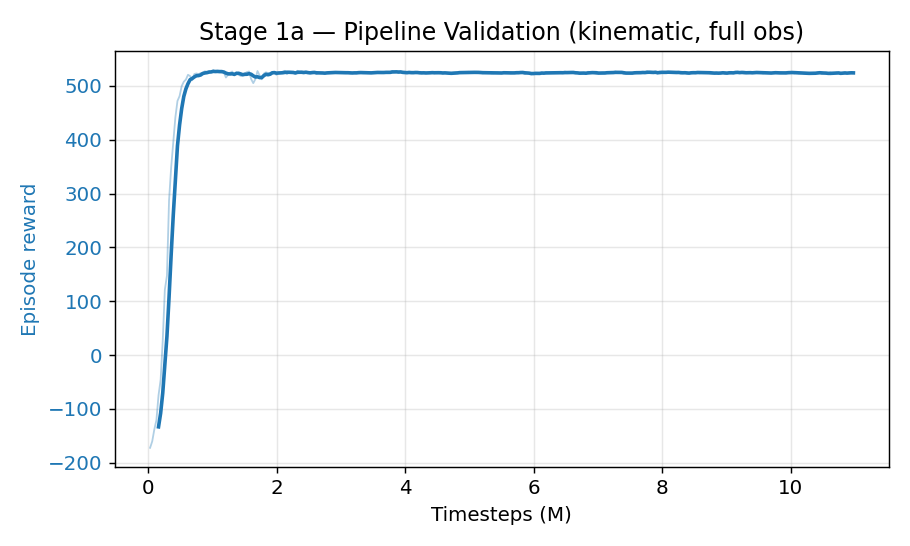
\includegraphics[width=\linewidth]{stage_1a/learning_curve.png}
\caption{Stage 1a learning curve.}\end{subfigure}\hfill
\begin{subfigure}{0.49\linewidth}\centering

\includegraphics[width=\linewidth]{stage_1b/learning_curve.png}
\caption{Stage 1b (acceleration control).}\end{subfigure}
\caption{Stages 1a--1b reward curves (smoothed). Rapid, stable convergence
confirms a correct pipeline.}
\label{fig:1a_curve}
\end{figure}

\subsection{Rich Visualizations \& Behavioral Analytics}
\begin{figure}[H]\centering
\begin{subfigure}{0.49\linewidth}\centering
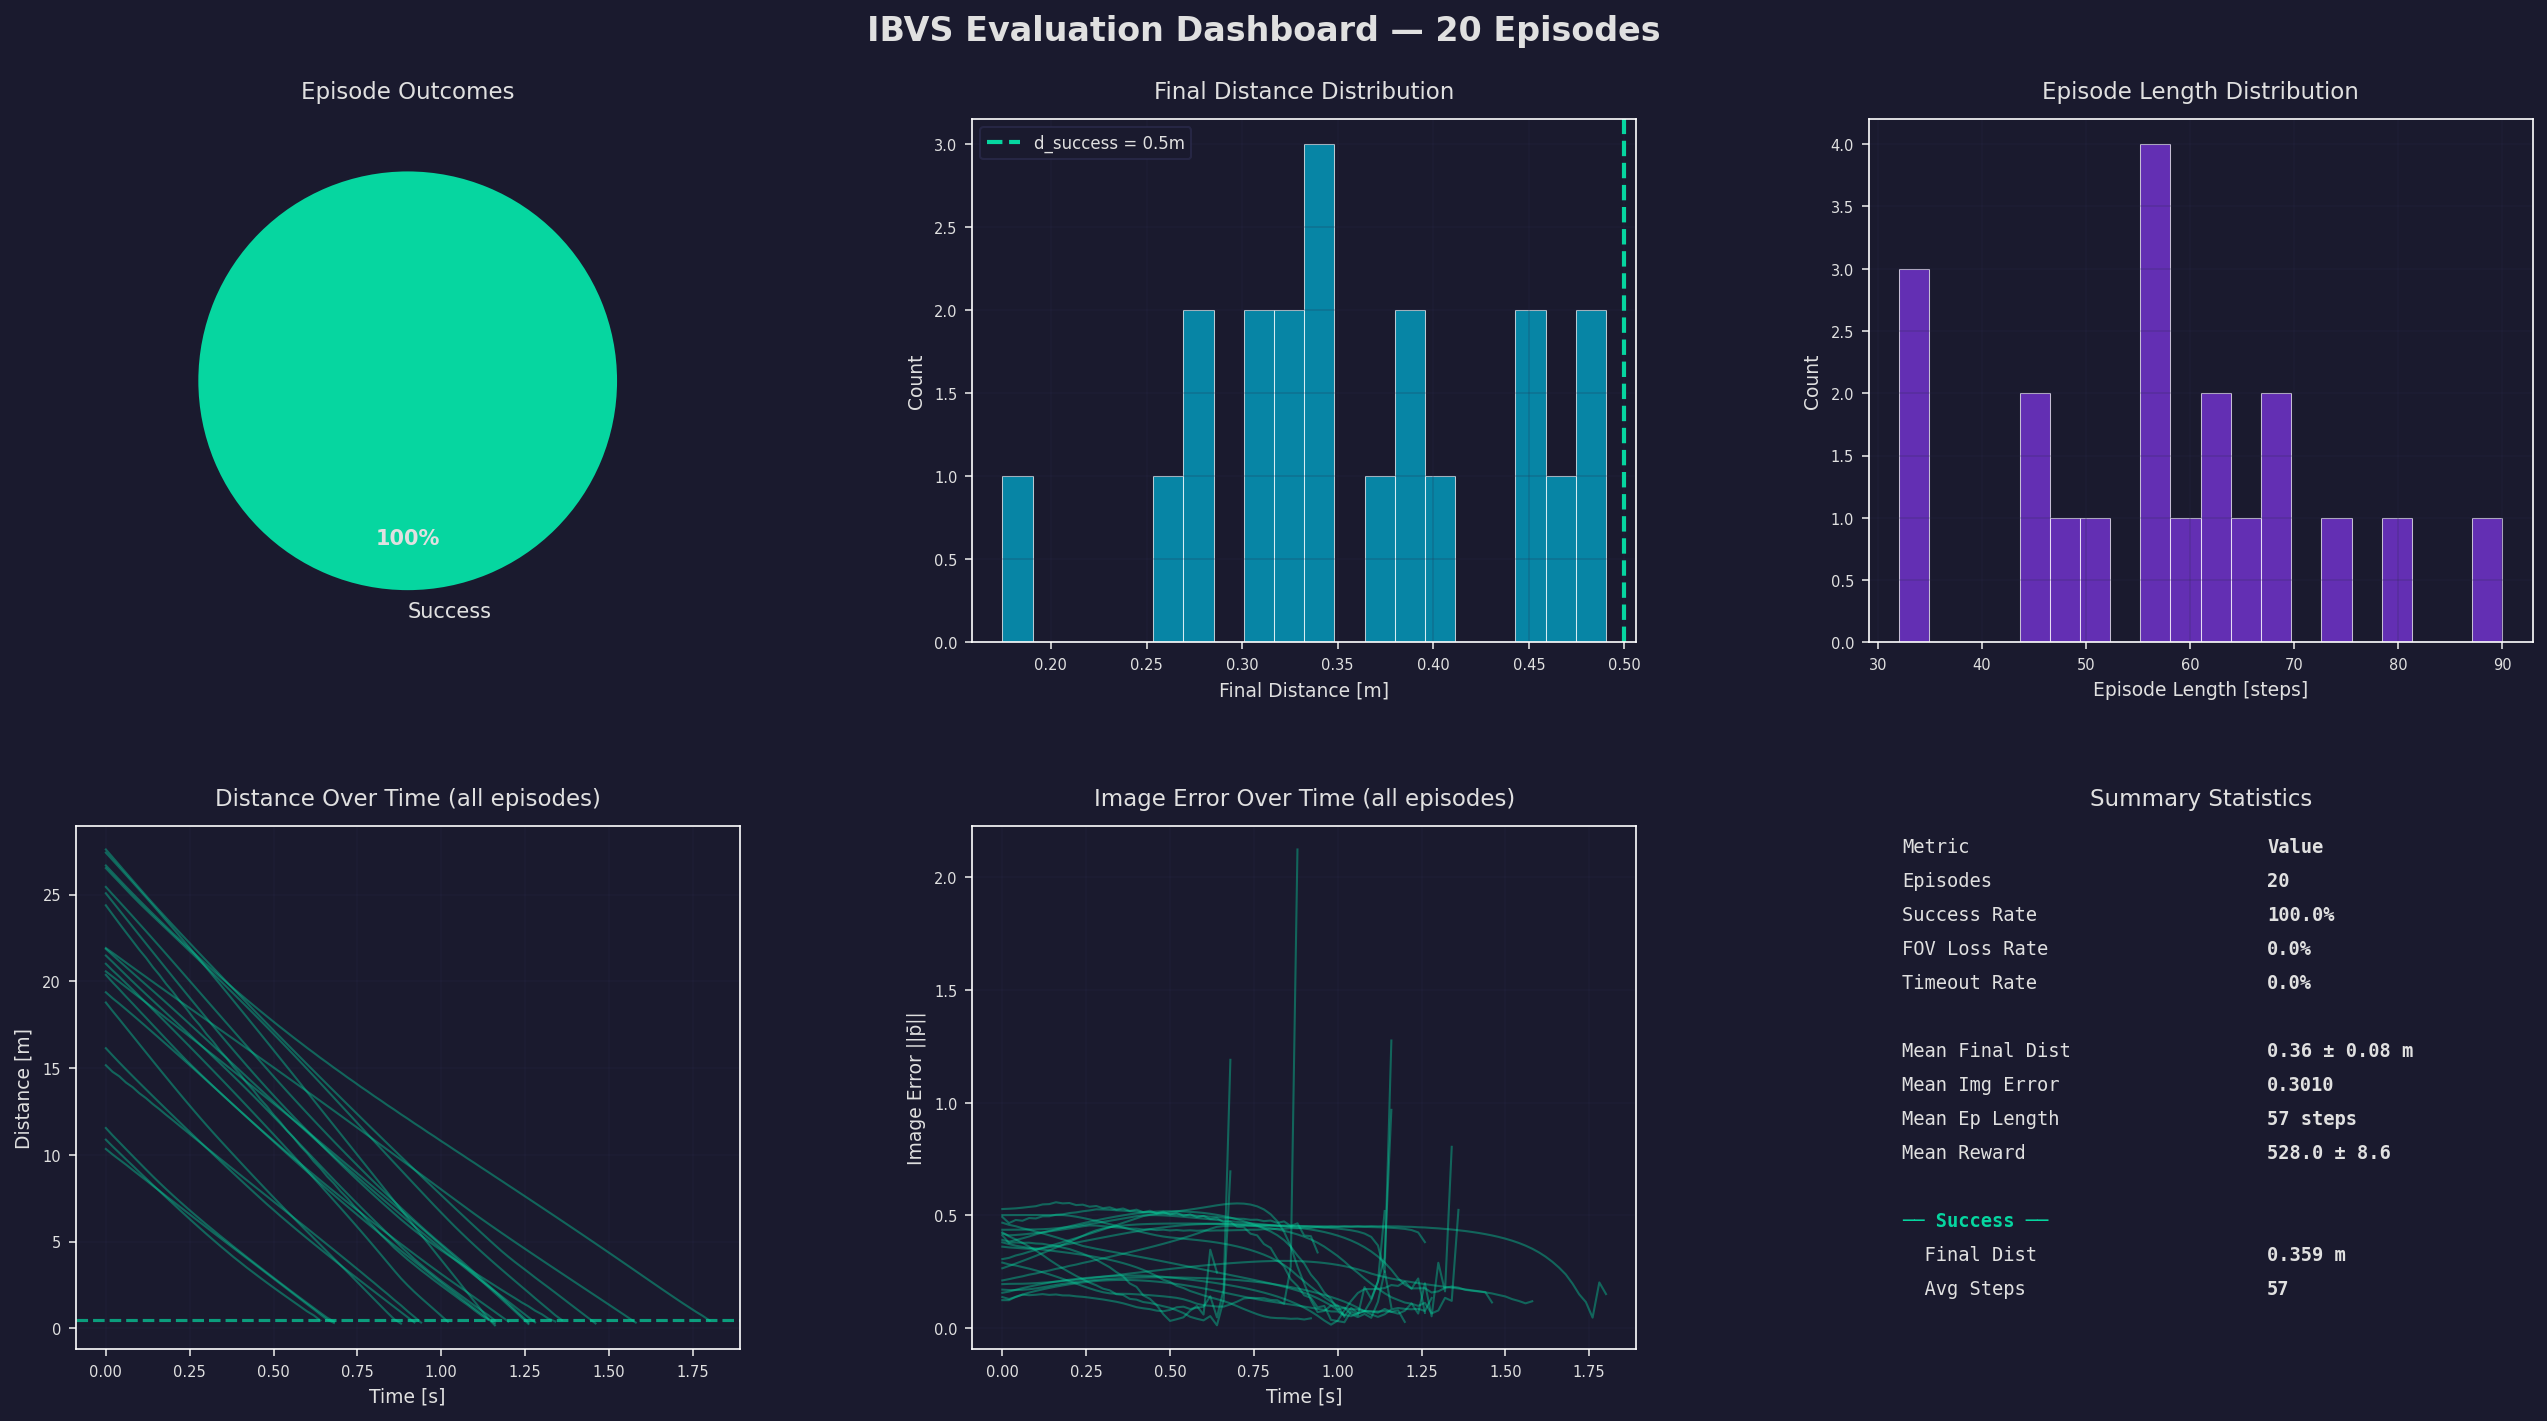
\includegraphics[width=\linewidth]{stage_1a/dashboard.png}
\caption{Aggregate 100-episode dashboard.}\end{subfigure}\hfill
\begin{subfigure}{0.49\linewidth}\centering
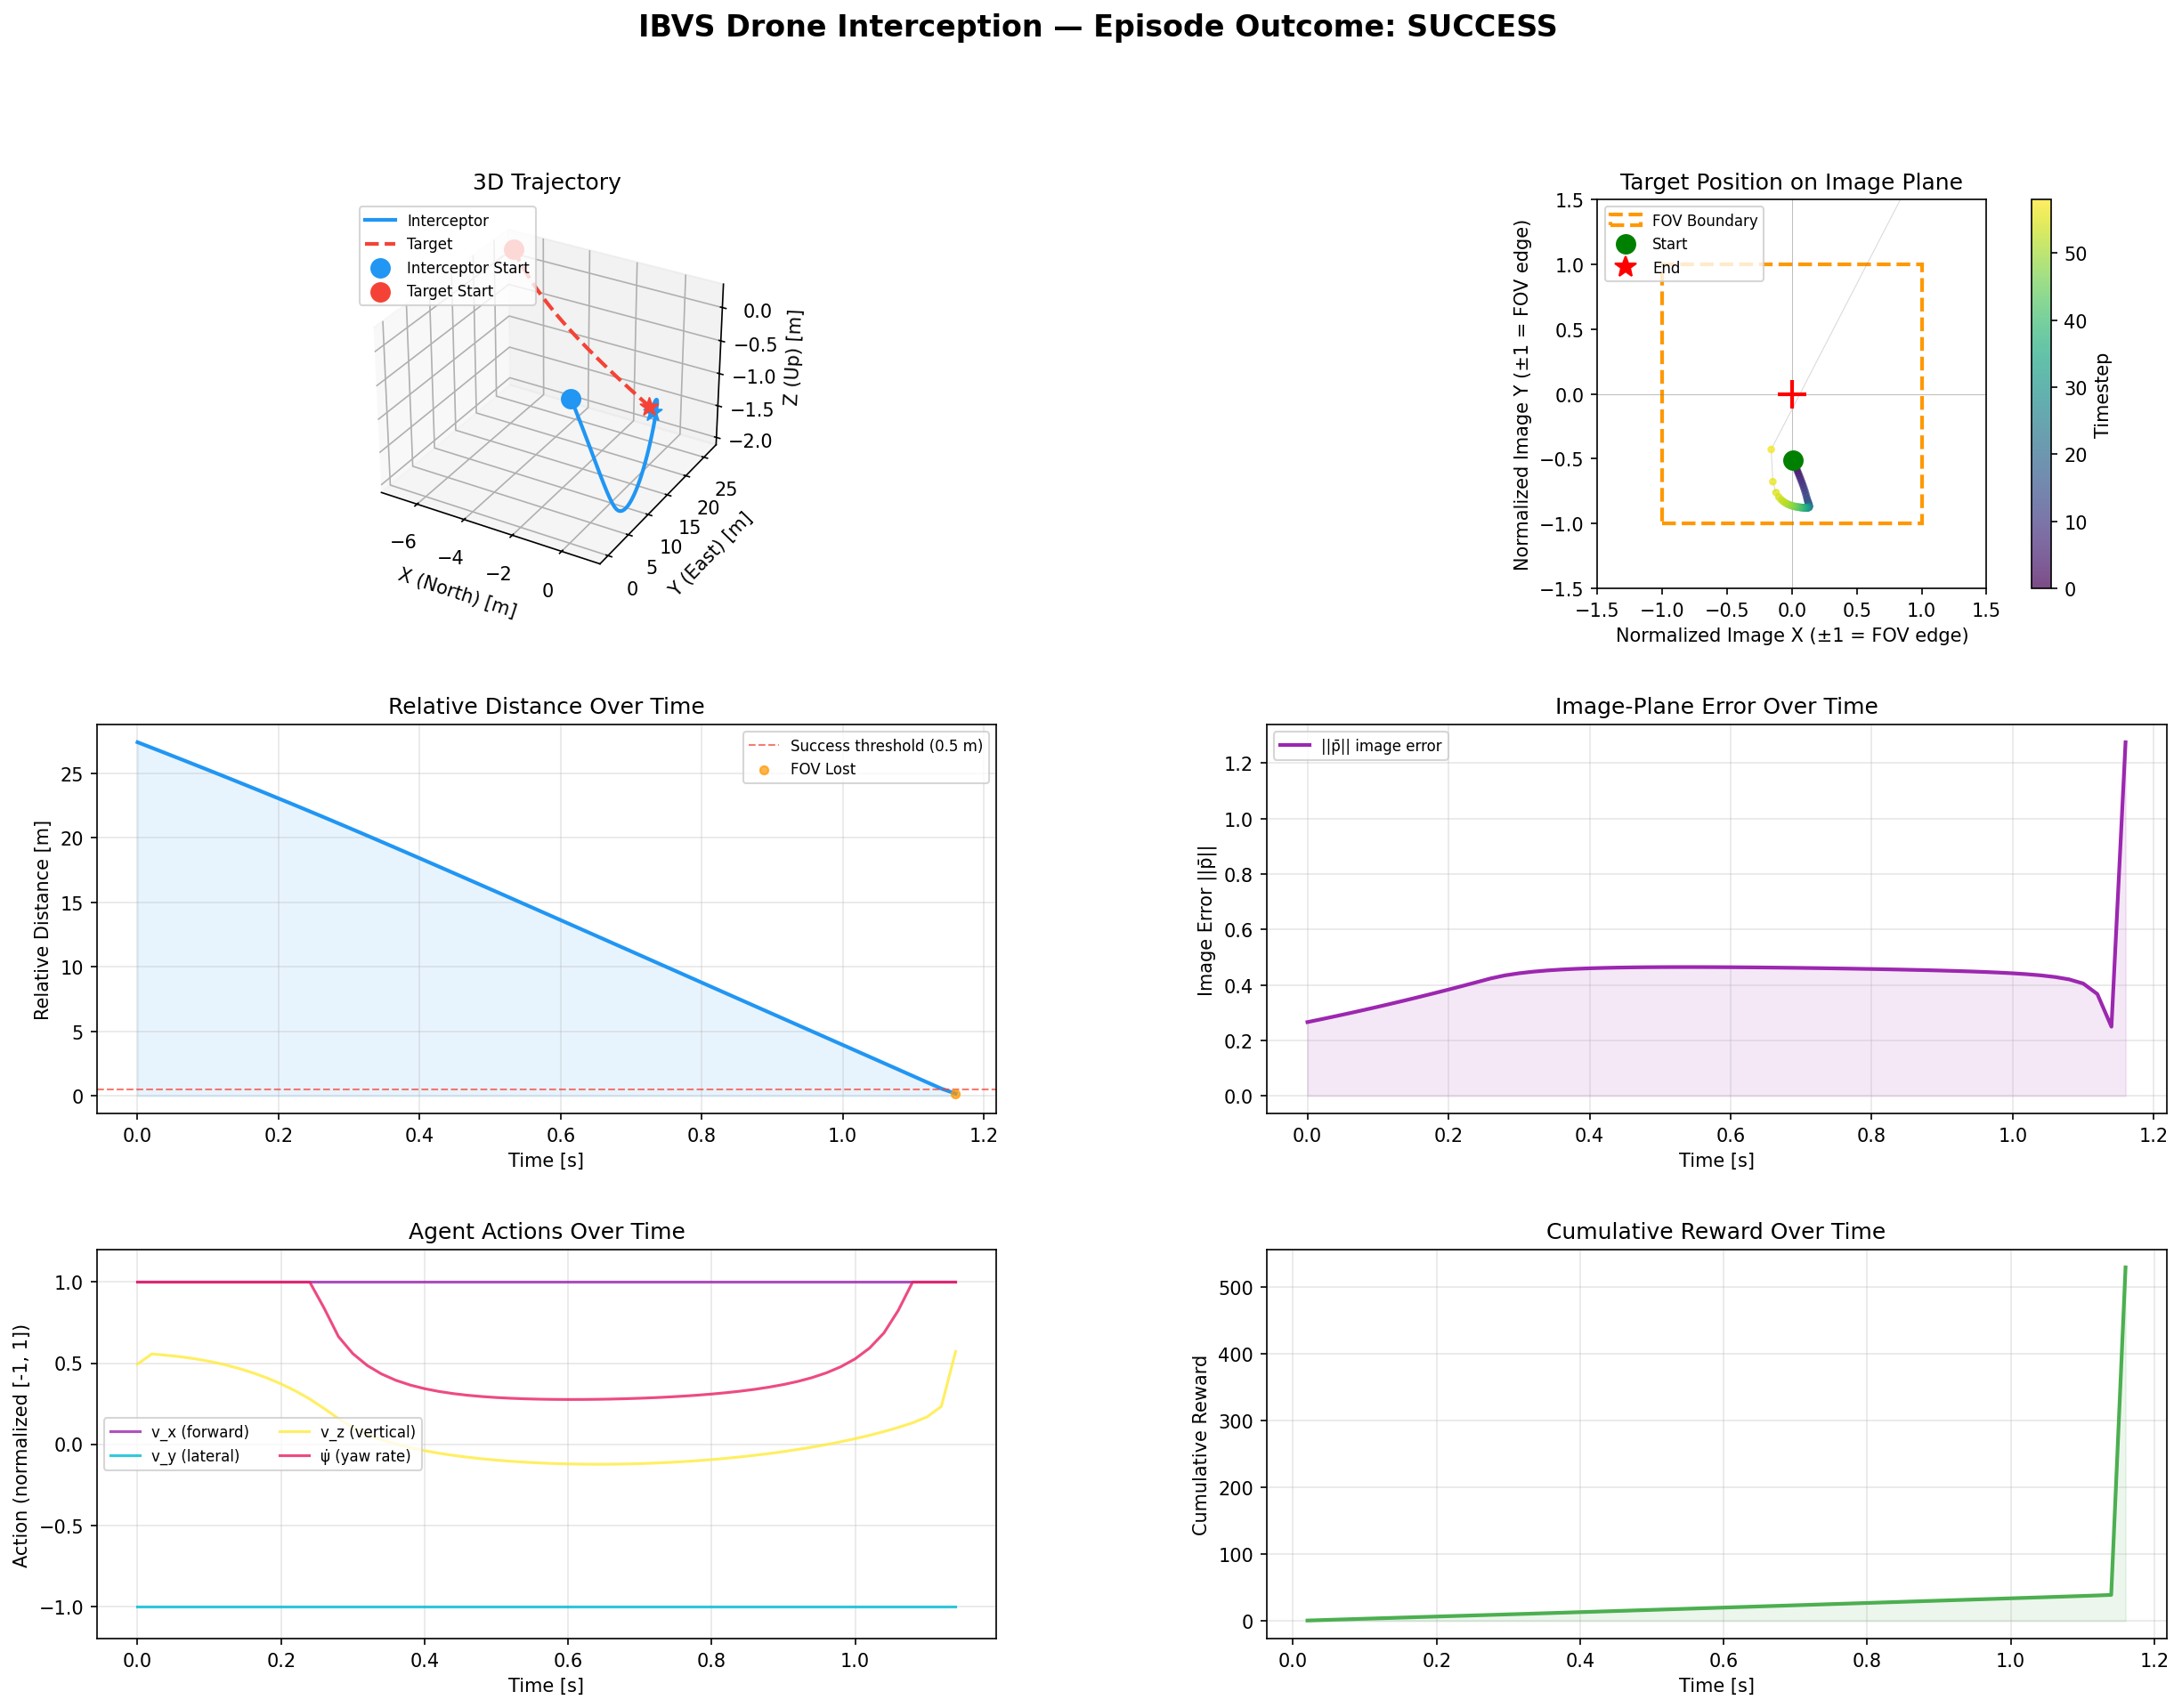
\includegraphics[width=\linewidth]{stage_1a/episode_analysis.png}
\caption{Single-episode multi-panel analysis.}\end{subfigure}
\caption{Stage 1a behavioral analytics: 3-D trajectory, image-plane error,
relative distance, reward, and action traces.}
\end{figure}

% =====================================================================
\section{Stage 2a--2b: Vision-Only Observation and the DKF Observer}
% =====================================================================
\subsection{Theoretical \& Algorithmic Foundations}
Stage 2a removes all privileged state, leaving a 16-D vision-only observation
(image position/velocity, in-FOV flag, depth estimate, attitude, previous
action). Stage 2b injects measurement noise and a delay of $D$ steps, then
inserts a \textbf{Disturbance Kalman Filter} (DKF): a 4-D image-plane filter
with state $[\bar p_x,\bar p_y,\dot{\bar p}_x,\dot{\bar p}_y]$ that compensates
both noise and delay. An IMU-aware prediction step feeds the ego-motion
contribution $\mathbf L_s[\mathbf v_\text{cam};\bm\omega_\text{cam}]$ forward,
sharpening the current-state estimate.

\stagebox{\textbf{Causal chain (\S\ref{sec:causal}):} sense $\rightarrow$
(2b) noise+delay $\rightarrow$ \emph{DKF estimate} (\S\ref{sec:dkf}) replaces
the raw image state $\rightarrow$ 16-D vision-only observation
(\S\ref{sec:state}, \S\ref{sec:depth} depth estimate; \emph{privileged $d$,
LOS, $\mathbf v_\text{rel}$ removed}) $\rightarrow$ policy $\rightarrow$
kinematic actuation. \emph{No safety layer.} \textbf{Reward:} \eqref{eq:reward}
unchanged from 1b; the difficulty is purely observational (the reward still
sees privileged $d$, but the \emph{policy} no longer does).}

\subsection{Experimental Setup \& Training Protocols}
Stage 2a: fresh, 5--10M steps. Stage 2b: warm-started from 2a, 2--3M steps,
with the noise/delay wrapper ($D{=}1$, $\sigma{=}0.015$ mild) and DKF wrapper
in the stack.

\subsection{Comprehensive Data, Charts, and Metrics}
Removing privileged state drops success to $\sim$70\% (2a); adding
noise+delay and the DKF stabilizes at 62\% (2b mild). The DKF is essential:
without it, the delayed/noisy image estimate destabilizes the terminal
approach.

\begin{figure}[H]\centering
\begin{subfigure}{0.49\linewidth}\centering

\includegraphics[width=\linewidth]{stage_2a/learning_curve.png}
\caption{Stage 2a (vision-only).}\end{subfigure}\hfill
\begin{subfigure}{0.49\linewidth}\centering

\includegraphics[width=\linewidth]{stage_2b/learning_curve.png}
\caption{Stage 2b (+ noise/delay/DKF).}\end{subfigure}
\caption{Vision-only and noisy-observation reward curves.}
\end{figure}

\subsection{Rich Visualizations \& Behavioral Analytics}
\begin{figure}[H]\centering
\begin{subfigure}{0.40\linewidth}\centering
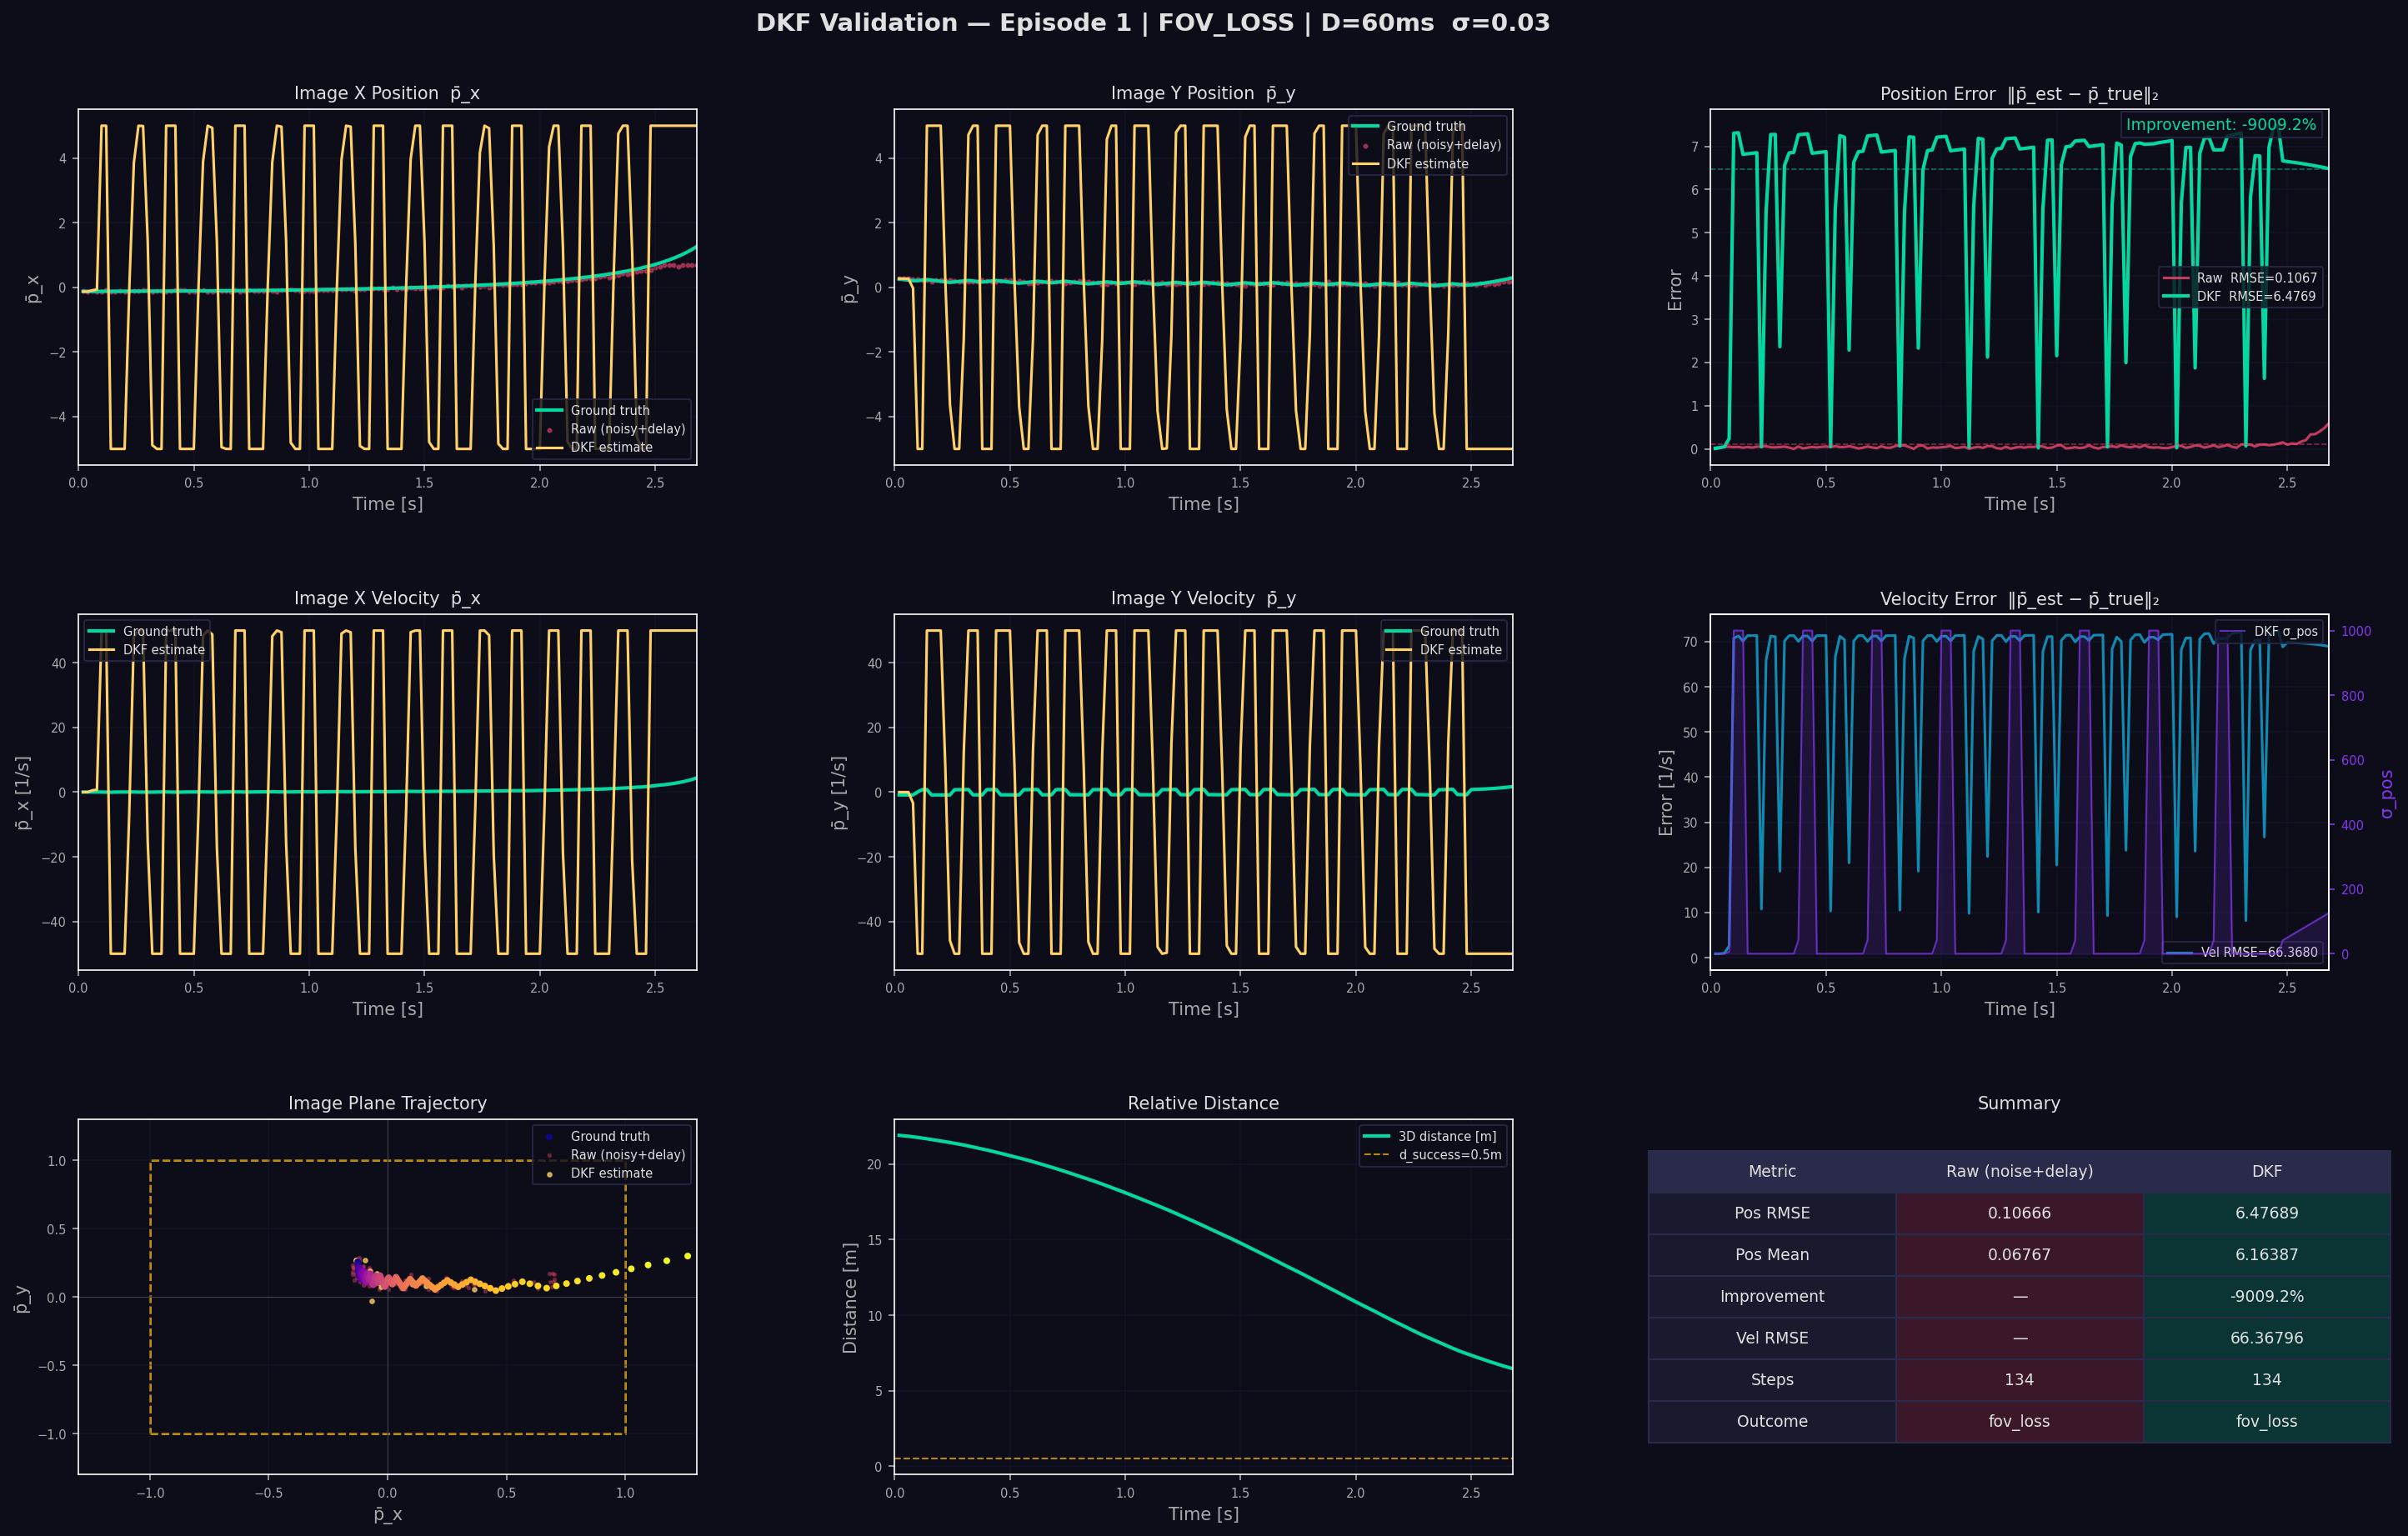
\includegraphics[width=\linewidth]{stage_2b/dkf_tracking.png}
\caption{DKF tracking vs noisy/delayed measurement.}\end{subfigure}\hfill
\begin{subfigure}{0.57\linewidth}\centering

\includegraphics[width=\linewidth]{stage_2b/dashboard.png}
\caption{Stage 2b aggregate dashboard.}\end{subfigure}
\caption{The DKF (left) recovers the true current image position from the
noisy, delayed stream, which is what makes the noisy regime trainable.}
\end{figure}

% =====================================================================
\section{Stage 3a: First-Order Dynamics and the Reward-Hacking Lesson}
\label{sec:3a}
% =====================================================================
\subsection{Theoretical \& Algorithmic Foundations}
Stage 3a adds first-order velocity lag ($\tau$) and attitude--camera coupling
(pitch $\approx-\arctan(a_x/g)$), so aggressive maneuvers tilt the camera and
risk FOV loss. The first attempt (v1) failed at 2\% deterministic success:
the policy discovered a \emph{reward-hacking} loiter --- backing off to
$>$40\,m to harvest image-centering reward while avoiding the FOV-loss risk of
committing. The fix (v2) was a distance-gated image reward
$r_\text{img}\!\cdot\!\max(0,1-d/d_\text{cut})$ plus an increased per-step
distance penalty, which makes loiter strictly dominated by commitment.

\stagebox{\textbf{Causal chain (\S\ref{sec:causal}):} sense+noise+delay
$\rightarrow$ IMU-aware DKF $\rightarrow$ 16-D obs $\rightarrow$ policy
$\rightarrow$ \emph{kinematic model (A), \S\ref{sec:dyn}}: the new
$\theta_\text{des}=-\arctan(a_x/g)$ coupling tilts the camera with
acceleration. \emph{No safety layer.} \textbf{Reward:} the canonical
\eqref{eq:reward} \emph{with} the distance gate
$\max(0,1-d/d_\text{cut})$, $d_\text{cut}=25\,$m, and $w_\text{dist}=-0.15$
(up from $-0.02$). \textbf{Reward-hacking analysis:} under the v1 weights, a
policy loitering at $35\,$m earned $\approx+0.24$/step image reward against
only $\approx-0.016$/step distance penalty (net $+0.17$/step) --- loiter
dominated commitment unless commit-success exceeded $\sim$66\%. The gate
zeroes image reward beyond $d_\text{cut}$, making $\approx-0.12$/step the only
steady-state option at range, so closure becomes the unique positive-return
strategy.}

\subsection{Experimental Setup \& Training Protocols}
Stage 3a-v2: fresh, 10--15M steps, clean observation. Stage 3a-noisy: warm,
2--5M steps, with mild noise + IMU-DKF. The IMU-aware DKF upgrade eliminated a
brake-penalty reward hack present in the constant-velocity DKF variant.

\subsection{Comprehensive Data, Charts, and Metrics}
\begin{table}[H]\centering\small
\caption{Stage 3a noise sensitivity (50-episode det.\ eval, kinematic model).}
\begin{tabular}{@{}lll@{}}
\toprule
Configuration & Observer & Success \\
\midrule
mild ($D{=}1,\sigma{=}.015$) & CV-DKF & 62\% \\
mild + brake polish & CV-DKF & 66\% \\
mild & IMU-DKF & 66\% \\
full ($D{=}3,\sigma{=}.03$) & CV/IMU-DKF & 0\% (collapsed) \\
\bottomrule
\end{tabular}
\end{table}
The full-noise collapse is a \emph{4-D DKF capacity limit}, not a dynamics or
reward issue --- it persists under 6-DOF (Stage 3b) and would require the
paper's 18-D EKF to resolve. Mild noise is therefore the canonical downstream
operating point.

\begin{figure}[H]\centering
\begin{subfigure}{0.49\linewidth}\centering
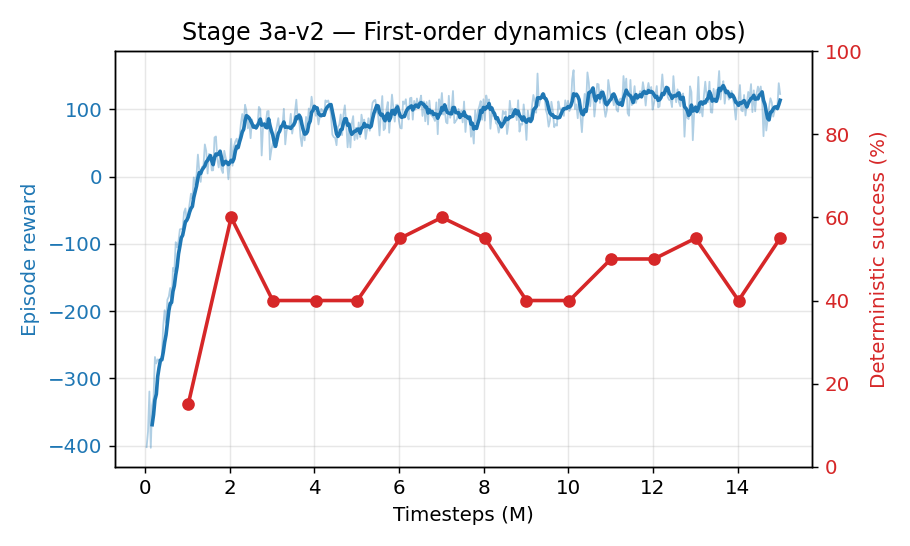
\includegraphics[width=\linewidth]{stage_3a/learning_curve_clean.png}
\caption{3a-v2 (clean).}\end{subfigure}\hfill
\begin{subfigure}{0.49\linewidth}\centering
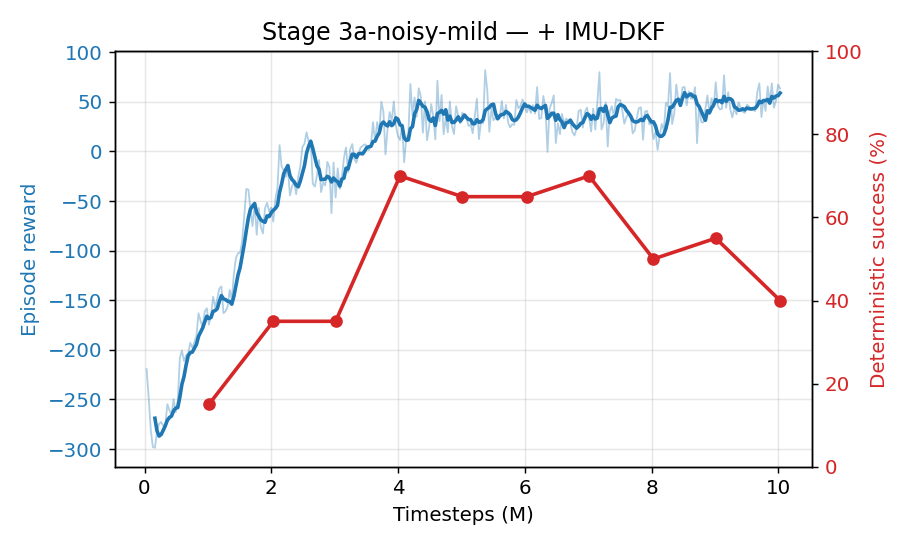
\includegraphics[width=\linewidth]{stage_3a/learning_curve_noisy.png}
\caption{3a-noisy-mild (+IMU-DKF).}\end{subfigure}
\caption{Stage 3a reward and deterministic success curves. The single-peak
success shape is the recurring overtraining pattern.}
\end{figure}

\subsection{Rich Visualizations \& Behavioral Analytics}
\begin{figure}[H]\centering
\begin{subfigure}{0.49\linewidth}\centering

\includegraphics[width=\linewidth]{stage_3a/episode_analysis.png}
\caption{Single-episode analysis.}\end{subfigure}\hfill
\begin{subfigure}{0.49\linewidth}\centering

\includegraphics[width=\linewidth]{stage_3a/replay_frame.png}
\caption{Mid-episode replay frame (animation in \texttt{stage\_3a/replay\_best.gif}).}
\end{subfigure}
\caption{Stage 3a interception behavior under first-order dynamics.}
\end{figure}

% =====================================================================
\section{Stage 3b: Full 6-DOF Dynamics and the SO(3) Attitude Controller}
\label{sec:3b}
% =====================================================================
\subsection{Theoretical \& Algorithmic Foundations}
Stage 3b replaces the kinematic model with full Newton--Euler translational
dynamics plus a geometric \textbf{SO(3) PD attitude controller}
(Lee et al.\ 2010), driven by a desired-thrust/desired-tilt construction:
the body acceleration command is lifted to EFCS, the required thrust vector
sets a desired rotation $R_d$, and the PD law
$\bm\omega_d=-k\,\mathrm{vex}(R_d^\top R - R^\top R_d)$ commands the body rate,
which is tracked through first-order motor/rate-loop lags. Quaternion
integration avoids Euler singularities at high tilt. The full controller and
Newton--Euler dynamics are derived in \S\ref{sec:so3} and \S\ref{sec:6dof}.

\stagebox{\textbf{Causal chain (\S\ref{sec:causal}):} sense+noise+delay
$\rightarrow$ IMU-aware DKF $\rightarrow$ 16-D obs $\rightarrow$ policy
$\mathbf a_b$ $\rightarrow$ \emph{SO(3) controller} \eqref{eq:so3} produces
$(f_d,\bm\omega_d)$ $\rightarrow$ first-order motor/rate loops $\rightarrow$
Newton--Euler integration \eqref{eq:newton} with quaternion attitude.
\emph{No safety layer yet.} \textbf{Reward:} canonical \eqref{eq:reward},
unchanged from 3a --- the gain comes entirely from dynamics fidelity, not
reward changes.}

\subsection{Experimental Setup \& Training Protocols}
Parameters: mass $1\,$kg, $J=\mathrm{diag}(0.01,0.01,0.02)$, $\tau_\text{motor}
=\tau_\text{rate}=50\,$ms, thrust-to-weight 3, $\omega_\text{max}=4\,$rad/s,
$k_\text{att}=6$. Stage 3b-clean: warm-started from 3a, 15M steps. Stage
3b-noisy-mild: + IMU-DKF, 5M steps.

\subsection{Comprehensive Data, Charts, and Metrics}
The dynamics upgrade produced a large, somewhat surprising gain:
\begin{table}[H]\centering\small
\caption{Stage 3b (200-ep det.\ eval, seed 1000).}
\begin{tabular}{@{}lll@{}}
\toprule
Configuration & Success & FOV-loss \\
\midrule
3b-clean (7M ckpt) & 96.0\% & --- \\
3b-noisy-mild + IMU-DKF (4M ckpt) & \textbf{96.5\%} & 3.5\% \\
3b-noisy-full + IMU-DKF & $\sim$2\% & (perception ceiling) \\
\bottomrule
\end{tabular}
\end{table}
The SO(3) controller yields \emph{smoother} attitude responses than the
kinematic $\arctan(a/g)$ coupling, so the policy keeps the target better
centered during aggressive terminal approach --- jumping from 66\% (kinematic
mild) to 96.5\% (6-DOF mild). Figure~\ref{fig:noise} contrasts the two models
across noise levels.

\begin{figure}[H]\centering
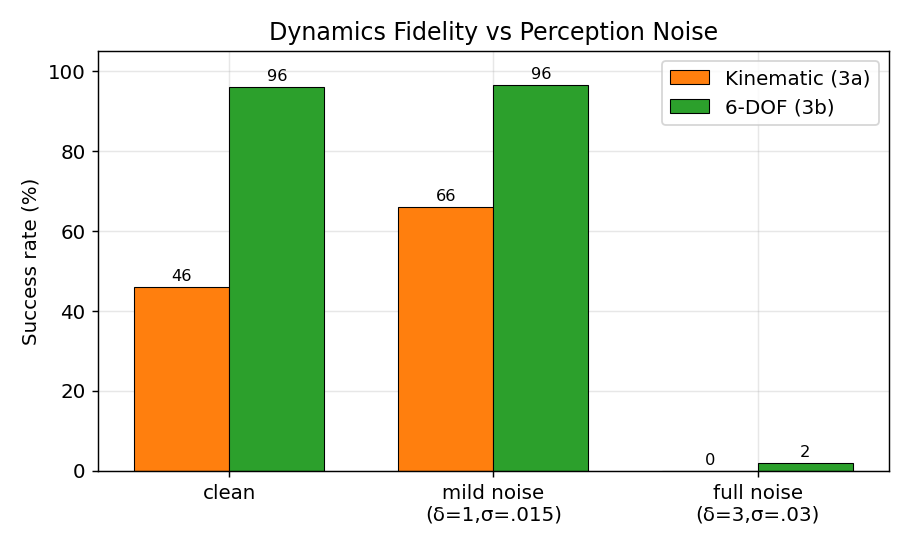
\includegraphics[width=0.72\linewidth]{figures/noise_sensitivity.png}
\caption{Dynamics fidelity vs perception noise. The 6-DOF model is far more
robust at mild noise; both collapse at full noise (4-D DKF ceiling).}
\label{fig:noise}
\end{figure}

\begin{figure}[H]\centering
\begin{subfigure}{0.49\linewidth}\centering

\includegraphics[width=\linewidth]{stage_3b/learning_curve_clean.png}
\caption{3b-clean.}\end{subfigure}\hfill
\begin{subfigure}{0.49\linewidth}\centering

\includegraphics[width=\linewidth]{stage_3b/learning_curve_noisy.png}
\caption{3b-noisy-mild.}\end{subfigure}
\caption{Stage 3b learning curves. Note the overtraining: deterministic
success peaks (4M) well before the final checkpoint.}
\end{figure}

\subsection{Rich Visualizations \& Behavioral Analytics}
\begin{figure}[H]\centering

\includegraphics[width=0.62\linewidth]{stage_3b/episode_analysis.png}
\caption{Stage 3b-noisy-mild single-episode analysis: smooth 6-DOF
interception with the target held near image center throughout.}
\end{figure}

% =====================================================================
\section{Stage 4a: Control-Barrier-Function Safety}
% =====================================================================
\subsection{Theoretical \& Algorithmic Foundations}
We enforce four safety constraints as CBFs $h_i(\mathbf x)\!\ge\!0$:
horizontal/vertical FOV preservation and pitch/roll limits, using the
squared form $h=(\text{limit})^2-(\cdot)^2$ (smooth, nonzero gradient at the
boundary). The classical CBF condition is
$L_f h(\mathbf x)+L_g h(\mathbf x)\mathbf u+\alpha\,h(\mathbf x)\ge0$,
an affine constraint in $\mathbf u$ suitable for a quadratic program (QP):
\[
\mathbf u_\text{safe}=\arg\min_{\mathbf u}\tfrac12\lVert\mathbf u-\mathbf u_\text{RL}\rVert^2
\quad\text{s.t.}\quad L_f h_i+L_g h_i\mathbf u\ge-\alpha_i h_i,\;\;\mathbf u\in[-1,1]^4.
\]
A subtlety drove the engineering: the FOV/attitude constraints are
relative-degree~2 in our action (acceleration $\rightarrow$ attitude lag
$\rightarrow$ image), so we use a control-affine \emph{proxy} linearization
(pitch tracks $-a_x/g$ with $\tau_\text{rate}$ lag) that renders all four
constraints relative-degree~1, giving closed-form Lie derivatives. The full
CBF construction --- barrier functions, Lie derivatives $L_f h_i$, $L_g h_i$,
the safe polytope $\mathcal C(\mathbf x)$, and the minimally-invasive QP
\eqref{eq:cbfqp} --- is derived in \S\ref{sec:cbf}.

\stagebox{\textbf{Causal chain (\S\ref{sec:causal}):} sense $\rightarrow$ DKF
$\rightarrow$ 16-D obs $\rightarrow$ policy $\mathbf u_\text{RL}$ $\rightarrow$
\emph{external CBF-QP} \eqref{eq:cbfqp} projects to
$\mathbf u_\text{safe}\in\mathcal C(\mathbf x)$ $\rightarrow$ SO(3) controller
$\rightarrow$ 6-DOF dynamics. \textbf{Reward:} canonical \eqref{eq:reward};
the safety layer is a \emph{post-hoc} action filter and does not alter the
reward. \textbf{Safety guarantee:} forward invariance of
$\{h_i\ge0\}$ under the relative-degree-1 proxy, with the inner margin
$\delta_s$ absorbing the proxy--truth gap (empirically $\le0.1\%$ attitude
exceedance).}

\subsection{Experimental Setup \& Training Protocols}
We evaluated four safety realizations:
\begin{description}[nosep,leftmargin=1.4em]
  \item[4a.1 Bisection bolt-on] action-magnitude line search over a 6-DOF
  rollout horizon; no retraining.
  \item[4a.2 Bisection co-trained] same filter inside the training loop, 3M
  steps + LR decay.
  \item[4a.3 HOCBF] proper analytical CBF-QP (quadprog) with an inner safety
  margin; eval-only on the locked 3b policy, then co-trained.
  \item[4a.4 HardNet] in-policy \emph{differentiable} CBF projection
  (\S\ref{sec:hardnet}).
\end{description}

\subsection{Comprehensive Data, Charts, and Metrics}
\begin{table}[H]\centering\small
\caption{Stage 4a safety-filter comparison (200-ep, seed 1000), nominal
operating point. Attitude exceedance = fraction of steps over the $0.611\,$rad
limit.}
\begin{tabular}{@{}llll@{}}
\toprule
Method & Success & FOV-loss & Attitude exceedance \\
\midrule
baseline (no CBF) & 96.5\% & 3.5\% & 9--39\% (unsafe) \\
4a.1 bisection bolt-on & 84.0\% & 16.0\% & 0\% \\
4a.2 bisection co-trained & 85.5\% & 14.5\% & 0\% \\
4a.3 HOCBF & \textbf{89.0\%} & 11.0\% & $\sim$0\% \\
\bottomrule
\end{tabular}
\end{table}
The bisection filter can only \emph{scale} the action (no redirection), so it
over-corrects ($\sim$80\% of steps) and caps success near 85\%. The analytical
HOCBF-QP redirects the action minimally (55\% correction rate, $0.36$ avg
norm), recovering to 89\% --- and runs in $0.15\,$ms/step, 60$\times$ faster
than the bisection's rollout predictor. All CBF methods reduce attitude
violations from $\sim$30\% of steps to $\le0.1\%$.

\begin{figure}[H]\centering
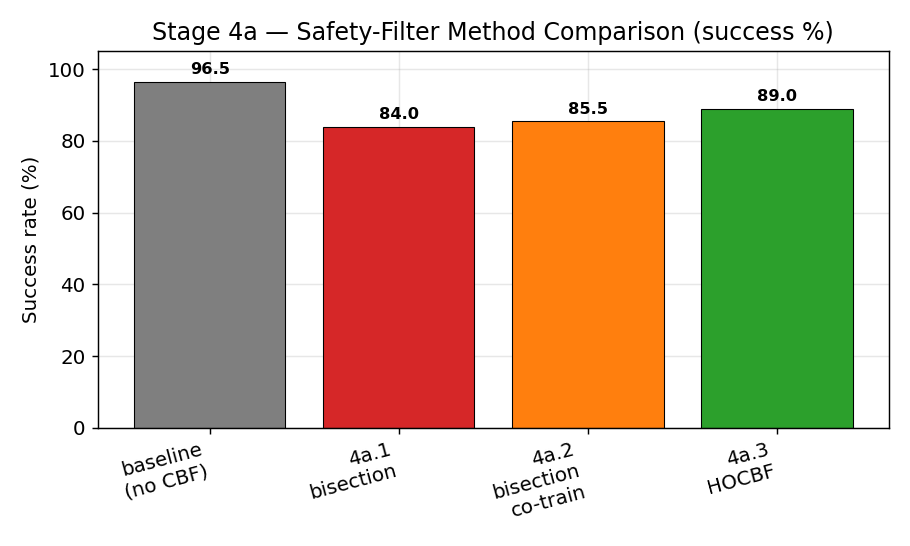
\includegraphics[width=0.72\linewidth]{figures/cbf_methods.png}
\caption{Stage 4a method comparison. The proper HOCBF-QP (green) closes most
of the gap the bisection filters could not.}
\end{figure}

\begin{figure}[H]\centering
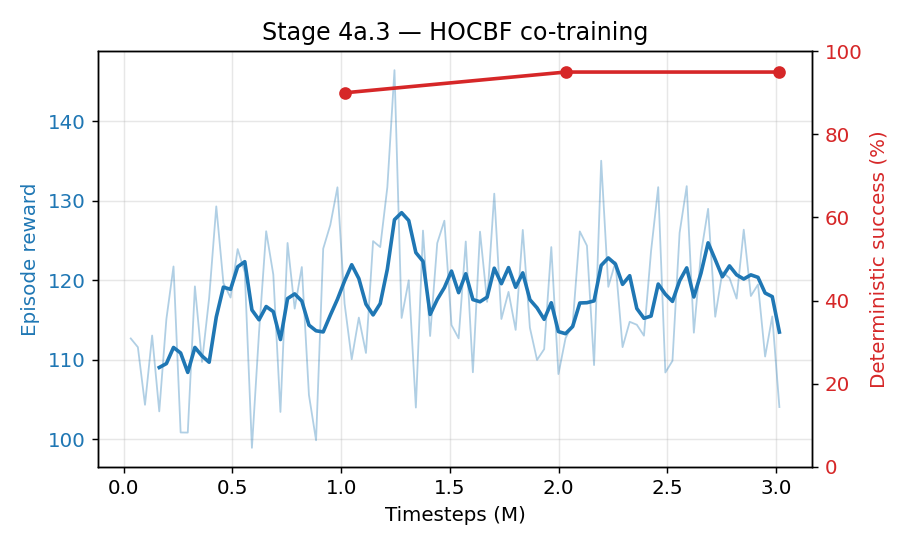
\includegraphics[width=0.62\linewidth]{stage_4a/learning_curve_hocbf.png}
\caption{HOCBF co-training learning curve.}
\end{figure}

\subsection{Rich Visualizations \& Behavioral Analytics}
\begin{figure}[H]\centering

\includegraphics[width=0.62\linewidth]{stage_4a/episode_analysis.png}
\caption{HOCBF-filtered interception: the safety filter keeps pitch/roll
strictly within limits while the policy pursues the target.}
\end{figure}

% =====================================================================
\section{Stage 4a.4: HardNet --- In-Policy Differentiable CBF Projection}
\label{sec:hardnet}
% =====================================================================
\subsection{Theoretical \& Algorithmic Foundations}
HardNet embeds the CBF projection \emph{inside} the policy network:
\[
\text{net}\rightarrow\mathbf u_\text{raw}\;\xrightarrow{\text{projection}}\;
\mathbf u_\text{safe}=\Pi_{\mathcal C(\mathbf x)}(\mathbf u_\text{raw}),
\]
where $\mathcal C(\mathbf x)=\{\mathbf u: A\mathbf u\ge b,\,\mathbf u\in[-1,1]^4\}$
is the per-step safe polytope (CBF half-spaces $\cap$ action box). The
projection is a differentiable Dykstra alternating projection, so gradients
flow \emph{through} the safe-set projection during PPO --- the policy learns
the constraint geometry rather than being corrected post-hoc. Crucially, the
executed and reward-relevant action is always $\mathbf u_\text{safe}$, so the
projection cannot induce unsafe or nonsensical behavior; it only reshapes the
network's internal pre-image. The per-step constraint coefficients $(A,b)$ are
appended to the observation (16$\rightarrow$36-D) by a context wrapper. The
Dykstra projection operator, its differentiability, and the auxiliary
feasibility loss are formalized in \S\ref{sec:hardnetmath}.

\stagebox{\textbf{Causal chain (\S\ref{sec:causal}):} sense $\rightarrow$ DKF
$\rightarrow$ 16-D obs $+$ CBF coefficients $(A,\mathbf b)$
$\rightarrow$ 36-D obs $\rightarrow$ policy emits $\mathbf u_\text{raw}$
$\rightarrow$ \emph{in-policy Dykstra projection}
$\mathbf u_\text{safe}=\Pi_{\mathcal C(\mathbf x)}(\mathbf u_\text{raw})$
(\S\ref{sec:hardnetmath}, gradients flow through) $\rightarrow$ SO(3)
controller $\rightarrow$ 6-DOF dynamics. \textbf{Reward:} canonical
\eqref{eq:reward} on the executed $\mathbf u_\text{safe}$, \emph{plus} the
auxiliary feasibility loss $\lambda\lVert\mathbf u_\text{raw}-\mathbf u_\text{safe}\rVert^2$
added to the PPO objective (Intervention D). \textbf{Key distinction from
4a.3:} safety is intrinsic to the policy (a differentiable layer), not an
external filter --- so the policy \emph{learns} the constraint geometry rather
than being corrected after the fact.}

\subsection{Experimental Setup \& Training Protocols}
HardNet warm-starts from the Stage 4b policy (all 13 weight tensors transfer,
since the network conditions only on the 16-D base observation via a slicing
extractor). Trained 3M steps on the full domain-randomized stack. The initial
single-seed run gave a \emph{mixed} verdict (HardNet won nominal but lost
worst-case to the external filter), which motivated a controlled robustness
study.

\subsection{Comprehensive Data, Charts, and Metrics: The Robustness Study}
We evaluate at three difficulty conditions through the full Stage 4b stack:
\textbf{nominal} ($\sigma{=}1.0$, $\sim$50\% detector dropout),
\textbf{hard} ($\sigma{=}1.5$, $\sim$75\%), \textbf{worst}
($\sigma{=}1.5$, $\sim$92\%).

\paragraph{Plan A --- variance baseline (3 seeds).} Worst-case degradation is
\emph{systematic} (all seeds $\sim$24\%), but the capacity exists (one seed
reached a 31\% worst-case ceiling). Nominal is reproducibly $91.6\%\pm2.2$.

\paragraph{Interventions C+B (negative result).} Capping the action standard
deviation ($\le1.0$) + lowering entropy + curriculum domain randomization
\emph{reduced} performance (worst $24.2\rightarrow21.2\%$). This
\textbf{rules out exploration instability} as the bottleneck: the std blow-up
was a symptom, not the cause.

\paragraph{Intervention D (positive result).} An auxiliary feasibility loss
$\mathcal L\mathrel{+}=\lambda\lVert\mathbf u_\text{raw}-\mathbf u_\text{safe}\rVert^2$
conditions the gradients (drives the projection toward identity, restoring a
full-rank Jacobian). This recovered worst-case to $33.9\%\pm4.3$ ($+9.7$pp)
with \emph{unchanged} nominal ($91.2\%$) and improved safety --- and now
\textbf{beats the external HOCBF filter at every condition.}

\begin{table}[H]\centering\small
\caption{HardNet robustness study (200-ep, seed 1000; means over 3 seeds).}
\begin{tabular}{@{}lccc@{}}
\toprule
 & Nominal & Worst (all-ckpt) & Worst ceiling \\
\midrule
baseline HardNet & 90.2\% & 24.2\% & 31\% \\
C+B (entropy+curriculum) & 85.2\% & 21.2\% & 24\% \\
\textbf{D (feasibility loss)} & \textbf{88.7\%} & \textbf{33.9\%} & \textbf{40\%} \\
external HOCBF filter & 91.0\% & 31.5\% & 31.5\% \\
\bottomrule
\end{tabular}
\end{table}

\begin{figure}[H]\centering
\begin{subfigure}{0.49\linewidth}\centering
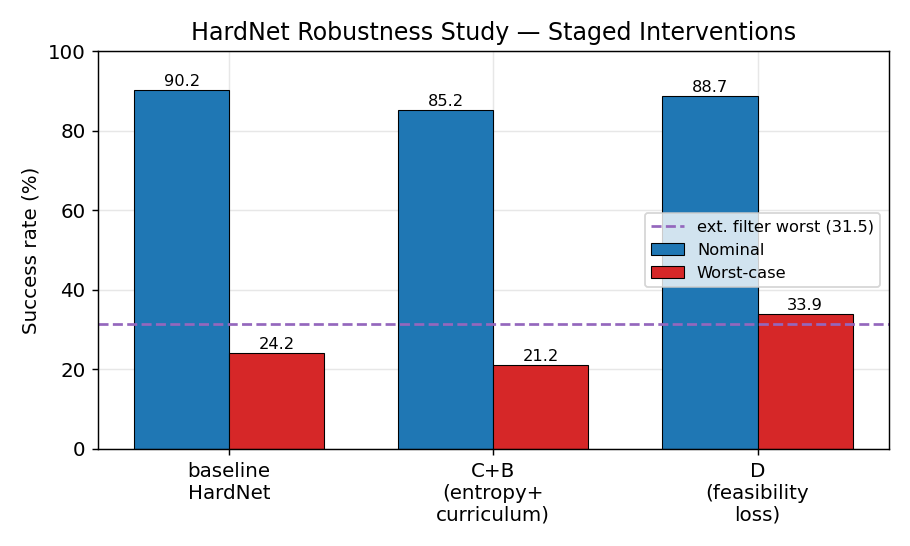
\includegraphics[width=\linewidth]{figures/intervention_arc.png}
\caption{Staged interventions.}\end{subfigure}\hfill
\begin{subfigure}{0.49\linewidth}\centering
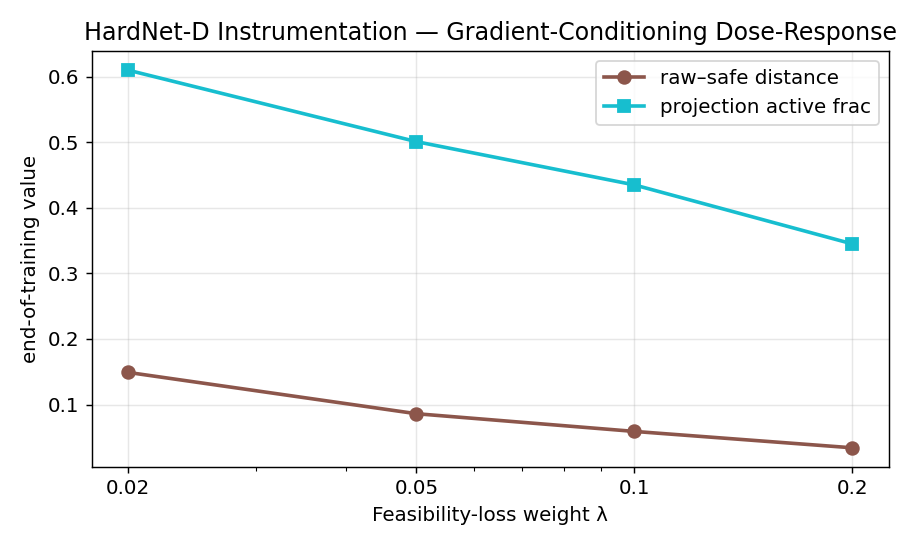
\includegraphics[width=\linewidth]{figures/hardnet_instrumentation.png}
\caption{Gradient-conditioning dose-response.}\end{subfigure}
\caption{Left: C+B hurts, D recovers and beats the filter. Right:
instrumentation confirms the mechanism --- higher $\lambda$ monotonically
drives $\lVert\mathbf u_\text{raw}-\mathbf u_\text{safe}\rVert$ down and the
projection toward identity.}
\end{figure}

\paragraph{$\lambda$ ablation.} Sweeping $\lambda\in\{0.02,0.05,0.1,0.2\}$
(3 seeds each) reveals a Pareto frontier: \emph{every} $\lambda$ beats both
baselines, worst-case is flat over $[0.02,0.1]$ then rises to $36.7\%$ at
$\lambda{=}0.2$, where a $\sim$3pp nominal cost (the ``lazy policy'' effect)
finally appears. For worst-case-priority (hardware) deployment, $\lambda{=}0.2$
is preferred; for balanced operation, $\lambda{=}0.05$.

\begin{figure}[H]\centering
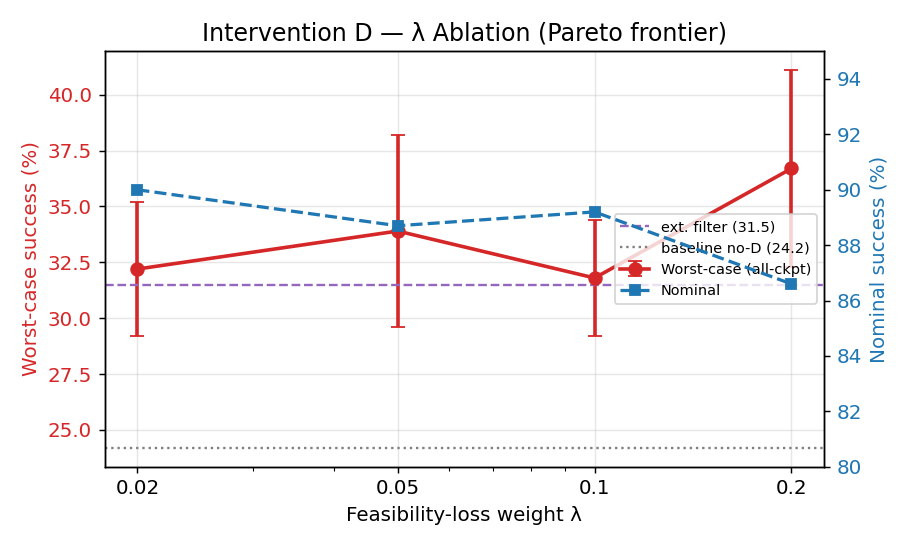
\includegraphics[width=0.72\linewidth]{figures/lambda_ablation.png}
\caption{Intervention D $\lambda$ ablation. Red = worst-case (with std),
blue = nominal. The lazy-policy trade-off appears only at $\lambda{=}0.2$.}
\end{figure}

\subsection{Rich Visualizations \& Behavioral Analytics}
\begin{figure}[H]\centering
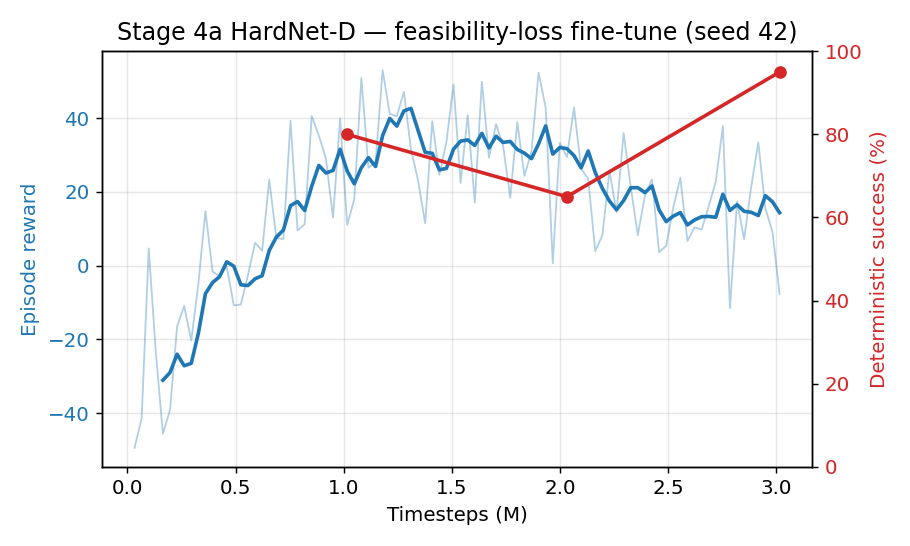
\includegraphics[width=0.62\linewidth]{stage_4a/learning_curve_hardnet_d.png}
\caption{HardNet-D fine-tune (seed 42). The feasibility term reshapes the raw
output distribution while task reward is preserved.}
\end{figure}

% =====================================================================
\section{Stage 4b: Realistic Perception and Wind Disturbance}
% =====================================================================
\subsection{Theoretical \& Algorithmic Foundations}
Stage 4b replaces perfect point detection with an intermittent detector
$p_\text{detect}=\sigma(\beta_1/d-\beta_2(1-m_\text{FOV})+\beta_3)$
(dropout grows with distance and FOV-edge proximity) and adds an
Ornstein--Uhlenbeck wind process coupled through linear drag
$\mathbf a_\text{drag}=-k(\mathbf v-\mathbf v_\text{wind})$. The DKF naturally
rides out missed detections via prediction-only steps. Domain randomization
(DR) over wind and detection parameters trains a single robust policy.

\stagebox{\textbf{Causal chain (\S\ref{sec:causal}):} sense $\rightarrow$
\emph{intermittent detector} (drop with prob.\ $1-p_\text{detect}$)
$\rightarrow$ noise+delay $\rightarrow$ DKF (prediction-only on dropped frames)
$\rightarrow$ 16-D obs $\rightarrow$ policy $\rightarrow$ CBF/HardNet safety
$\rightarrow$ SO(3) controller $\rightarrow$ 6-DOF dynamics \emph{plus wind
drag} $\mathbf a_\text{drag}=-k(\mathbf v-\mathbf v_\text{wind})$, with
$\mathbf v_\text{wind}$ an Ornstein--Uhlenbeck process
$d\mathbf v_\text{wind}=-\vartheta\,\mathbf v_\text{wind}\,dt+\varsigma\,d\mathbf W$.
\textbf{Reward:} canonical \eqref{eq:reward}. \textbf{Training:} domain
randomization samples $(\varsigma,\vartheta,k)$ and detector
$(\beta_1,\beta_2,\beta_3)$ per episode from the hard band, so a single policy
generalizes across the disturbance range.}

\subsection{Experimental Setup \& Training Protocols}
Warm-started from 3b, 5M steps, full hard DR band
($\sigma_\text{wind}\in[0,2]$, $\beta_3\in[-1,2]$), HOCBF in the loop,
linear LR decay.

\subsection{Comprehensive Data, Charts, and Metrics}
DR training is a decisive win over the non-DR baseline:
\begin{table}[H]\centering\small
\caption{Stage 4b vs locked 3b policy through the 4b stack (200-ep, seed 1000).}
\begin{tabular}{@{}llll@{}}
\toprule
Condition (detector drop) & 4b (DR) & 3b (no DR) & $\Delta$ \\
\midrule
nominal ($\sim$50\%) & \textbf{91.0\%} & 76.5\% & $+14.5$ \\
hard ($\sim$75\%) & 74.0\% & 51.0\% & $+23.0$ \\
worst ($\sim$92\%) & 31.5\% & 16.0\% & $+15.5$ \\
\bottomrule
\end{tabular}
\end{table}
All plan criteria are met: $>$30\% worst-case, graceful monotonic
degradation, and recovery from temporary detection loss.

\begin{figure}[H]\centering
\begin{subfigure}{0.49\linewidth}\centering
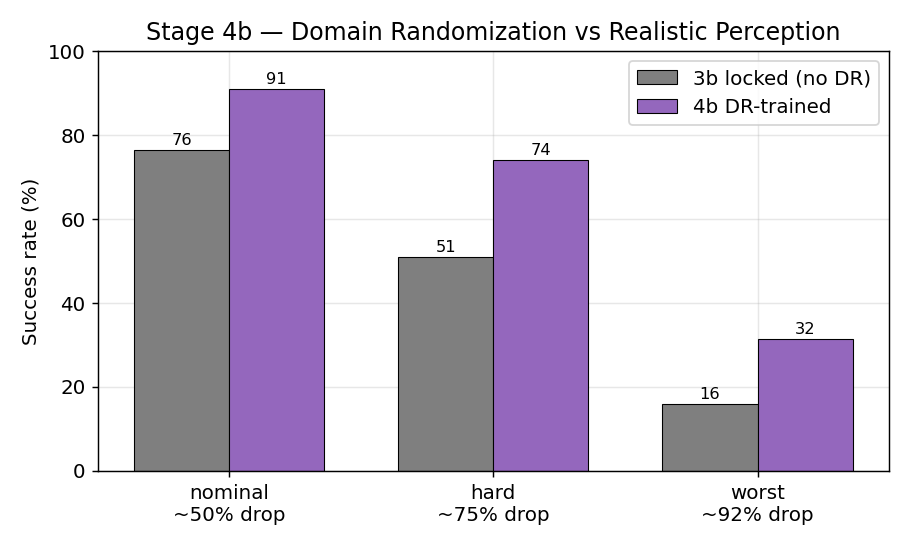
\includegraphics[width=\linewidth]{figures/stage4b_degradation.png}
\caption{DR vs no-DR across conditions.}\end{subfigure}\hfill
\begin{subfigure}{0.49\linewidth}\centering

\includegraphics[width=\linewidth]{stage_4b/learning_curve.png}
\caption{4b DR learning curve.}\end{subfigure}
\caption{Stage 4b: domain randomization buys 14--23pp under realistic
noise/wind for a $\sim$5pp disturbance-free cost.}
\end{figure}

\subsection{Rich Visualizations \& Behavioral Analytics}
\begin{figure}[H]\centering

\includegraphics[width=0.62\linewidth]{stage_4b/episode_analysis.png}
\caption{Stage 4b interception under wind + intermittent detection: the policy
rides out detection gaps (flat image-estimate segments) and re-acquires.}
\end{figure}

% =====================================================================
\section{Synthesis and Deployment Recommendation}
% =====================================================================
The study yields a single, defensible deployment configuration and a clear
research narrative:
\begin{itemize}[nosep]
  \item \textbf{Dynamics fidelity matters more than expected}: the
  kinematic$\rightarrow$6-DOF upgrade (3a$\rightarrow$3b) gave $+30$pp at mild
  noise via smoother SO(3) attitude responses.
  \item \textbf{Perception, not dynamics, is the ceiling}: full-noise collapse
  is a 4-D DKF limitation that an 18-D EKF would address (future work).
  \item \textbf{Safety can be free of nominal cost}: HardNet-D matches the
  unconstrained nominal success while guaranteeing attitude limits
  ($\le0.02\%$ exceedance) and \emph{improving} worst-case robustness.
  \item \textbf{In-policy projection $>$ external filter}, once gradients are
  conditioned (Intervention D): $36.7\%$ vs $31.5\%$ worst-case.
\end{itemize}

\stagebox{\textbf{Recommended deployable artifact:} HardNet-D at
$\lambda=0.2$ (locked: \texttt{stage4a\_hardnet\_d\_locked/ibvs\_ppo\_best\_lam02.zip},
$92.5\%$ nominal / $43.5\%$ worst at its checkpoint) for worst-case-priority
hardware deployment; $\lambda=0.05$ for balanced operation. A single
end-to-end differentiable policy --- no online QP at inference --- with hard
attitude-safety guarantees and graceful degradation from $91\%$ (nominal) to
$\sim$37\% (92\% detector dropout + $1.5\,$m/s wind).}

\paragraph{Scope and honest limitations.} This is a high-fidelity
\emph{simulation} study. Outstanding gaps before physical flight: a real
detector (vs.\ point-projection), full aerodynamics/rotor mixing, an IMU/GPS
sensor model, sim-to-real domain randomization beyond wind/detection, and a
PX4/MAVLink autopilot interface with a hard real-time C/C++ port of the
projection. These define the next phase (hardware bridge).

\end{document}
